\documentclass[10pt,a4paper]{article}

% ============================================================
% FORMATTAZIONE RICHIESTA DALLA CONSEGNA: Arial 10pt, interlinea singola
% ============================================================
\usepackage[utf8]{inputenc}
\usepackage[T1]{fontenc}
\usepackage{helvet}                  % Helvetica: sostituto metricamente equivalente ad Arial
\renewcommand{\familydefault}{\sfdefault}
\usepackage{geometry}
\geometry{a4paper, margin=2.2cm}
\usepackage{setspace}
\singlespacing

% ============================================================
% PACCHETTI PER TABELLE E FIGURE
% ============================================================
\usepackage{booktabs}
\usepackage{longtable}
\usepackage{array}
\usepackage{graphicx}
\usepackage{caption}
\usepackage{hyperref}
\hypersetup{colorlinks=true, linkcolor=black, urlcolor=blue, citecolor=black}
\usepackage[italian,nameinlink]{cleveref}
\usepackage{xcolor}
% \cref imposta internamente il colore a linkcolor (nero) perché colorlinks=true:
% un \textcolor esterno verrebbe sovrascritto. Si ridefinisce linkcolor localmente
% (in un gruppo) solo per la durata del riferimento.
\newcommand{\tabref}[1]{\textbf{\begingroup\hypersetup{linkcolor=red!70!black}\cref{#1}\endgroup}}
\usepackage{enumitem}
\setlist{nosep, itemsep=1pt}         
% Riduce lo spazio verticale attorno ai titoli di sezione (documento denso)
\usepackage{titlesec}
\titlespacing*{\section}{0pt}{8pt}{4pt}
\titlespacing*{\subsection}{0pt}{6pt}{3pt}

\title{\vspace{-1.5cm}Report di Progetto -- ISW2 Modulo 2\\[2pt]\large Software Testing su Apache Avro (fork \texttt{lucaaa02})}
\author{[Nome Cognome] -- [Matricola]}
\date{[Data]}

\begin{document}
\maketitle
\vspace{-1cm}
\pagenumbering{roman} 
\tableofcontents
\newpage
\pagenumbering{arabic} 
\setcounter{page}{1}
% ============================================================
% CAPITOLI -- un file per capitolo, dentro la cartella capitoli/
% Decommentare via via che i file vengono creati.
% ============================================================
% ============================================================
% CAPITOLO 1 -- INTRODUZIONE
% ============================================================
\section{Introduzione}

L'elaborato ha come obiettivo la realizzazione di un'attività di verifica
software su un fork di Apache Avro, applicata a due classi del progetto.

La verifica è stata condotta attraverso diverse metodologie di testing:
test manuali basati sulla tecnica Category-Partition, test generati
automaticamente tramite Randoop, test generati con l'ausilio di un LLM,
e test guidati dalla copertura tramite EvoSuite.

Sono stati isolati i test relativi alle due classi in esame, escludendo
dall'esecuzione la suite di test già presente nel progetto originale.

\subsection{Apache Avro}

Apache Avro è un framework di serializzazione dati, nato all'interno del
progetto Hadoop. Fornisce un formato binario compatto ed efficiente per
la codifica dei dati, un sistema di schemi (definiti in formato JSON) che
descrivono la struttura dei dati serializzati, e un meccanismo di
\emph{schema evolution}, ovvero la possibilità di far comunicare tra loro
versioni diverse dello stesso schema senza rompere la compatibilità.
Quest'ultimo aspetto è direttamente rilevante per il progetto: una delle
due classi analizzate (\texttt{Resolver}) implementa proprio la logica di
risoluzione tra schema \emph{writer} e schema \emph{reader}.

\subsection{Classi selezionate}

La selezione delle classi è avvenuta applicando l'algoritmo di
\emph{class ranking} descritto nella consegna, basato sull'iniziale del
cognome dello studente applicata alla classifica dei code smell rilevati
da SonarCloud sul progetto Apache Avro.

Una prima classe candidata, è stata scartata per banalità, in accordo con l'indicazione della consegna di evitare
classi il cui testing risulti banale o impraticabile, è stata selezionata la classe successiva.

Le classi definitivamente selezionate sono:
\begin{itemize}
    \item \texttt{org.apache.avro.Resolver} (473 LOC, 25 code smell):
    classe di utilità che confronta, ricorsivamente, l'albero dello
    schema usato da chi ha \emph{scritto} i dati (\emph{writer}) con
    l'albero dello schema atteso da chi li deve \emph{leggere}
    (\emph{reader}). Per ogni coppia di nodi corrispondenti, determina
    quale azione è necessaria per adattare i dati scritti al formato
    atteso in lettura (nessuna azione, promozione di tipo, adattamento
    di record/enum/union, oppure segnalazione di incompatibilità),
    producendo un albero di oggetti \texttt{Resolver.Action}. È il
    meccanismo alla base della \emph{schema evolution} di Avro, ovvero
    la capacità di far comunicare correttamente produttori e
    consumatori di dati che utilizzano versioni diverse dello stesso
    schema;
    \item \texttt{org.apache.avro.util.Utf8} (172 LOC, 8 code smell):
    classe mutabile che rappresenta una sequenza di testo codificata
    direttamente come array di byte UTF-8, anziché come \texttt{String}
    Java (rappresentata internamente in UTF-16). Implementa le
    interfacce \texttt{CharSequence}, \texttt{Comparable} ed
    \texttt{Externalizable}, fornendo metodi per impostare e leggere il
    contenuto, confrontare istanze e calcolarne l'hash. È utilizzata dal
    modello dati generico di Avro per rappresentare i campi di tipo
    stringa evitando le conversioni di codifica ripetute che
    sarebbero necessarie utilizzando \texttt{String}.
\end{itemize}
% ============================================================
% CAPITOLO 2 -- INFRASTRUTTURA DI PROGETTO
% ============================================================
\section{Infrastruttura di progetto}

\subsection{Build e gestione delle dipendenze}

Il progetto Avro è organizzato come progetto multi-modulo Maven, con un
file \texttt{pom.xml} principale che coordina i sotto-progetti, tra cui
il modulo \texttt{lang/java/avro/}, dove abbiamo lavorato, che contiene
le classi \texttt{Resolver} e \texttt{Utf8} selezionate per il testing.

È stato necessario l'utilizzo di tre versioni diverse del JDK: 11, 17 e
21. Il progetto Avro richiede infatti la compatibilità con JDK 11 per il
codice compilato; inoltre, Randoop ed EvoSuite, generando codice sulla
base della JVM su cui vengono eseguiti, devono essere lanciati anch'essi
con JDK 11, per evitare di generare riferimenti a metodi non disponibili
nella versione richiesta per la compilazione finale. Le versioni JDK 17
e 21 sono invece necessarie per compilare ed eseguire il progetto nelle
altre fasi della build.

\subsection{Integrazione continua e misurazione della copertura}

È stata configurata un'integrazione continua tramite GitHub Actions: ad
ogni \texttt{push} sul branch principale, il file di configurazione
\texttt{isw2-ci.yml} esegue automaticamente una serie di step, tra cui
la compilazione del progetto e l'esecuzione dei test su una macchina
virtuale remota. Per la misurazione della copertura è stato utilizzato
JaCoCo, analizzando le metriche di statement e branch coverage, mentre
SonarCloud è stato integrato come supporto per l'analisi della qualità
del codice.

L'integrazione continua si è rivelata utile per individuare problemi non
visibili nell'ambiente di sviluppo locale: in particolare, un conflitto
tra il JDK usato per la compilazione in CI (JDK 21) e il codice generato
da EvoSuite (eseguibile correttamente solo su JDK 11) si è manifestato
soltanto durante l'esecuzione su GitHub Actions.

Sono stati inoltre utilizzati Spotless e Apache RAT per garantire la
qualità del codice e la conformità alle licenze. Spotless applica
automaticamente le regole di formattazione del progetto (indentazione,
ordine degli import), mentre Apache RAT verifica che ogni file sorgente
contenga l'header di licenza Apache 2.0, in linea con le politiche della
Apache Software Foundation. Entrambi i controlli vengono eseguiti prima
della fase di test, durante la compilazione: un file che non li rispetta
blocca l'intera build, indipendentemente dal fatto che i suoi test
vengano poi effettivamente eseguiti. Poiché i file di test generati
automaticamente da Randoop ed EvoSuite non rispettano lo stile del
progetto né includono l'header di licenza, è stato necessario
configurare esclusioni esplicite per queste cartelle in entrambi gli
strumenti.

\subsection{Isolamento dei test del progetto}

L'esecuzione dei test già presenti nel progetto è stata disabilitata,
mantenendo attiva una suite di test composta unicamente dai test
sviluppati per questo lavoro.
% ============================================================
% CAPITOLO 3 -- TEST MANUALI (CATEGORY PARTITION)
% ============================================================
\section{Test manuali (Category Partition)}

La tecnica Category-Partition è un metodo di progettazione di test
black-box che procede in quattro fasi: identificazione dei domini di
input della funzionalità sotto test, a partire dalla documentazione o
dal comportamento atteso; derivazione, per ciascun dominio, delle
classi di equivalenza, ovvero sottoinsiemi di valori per cui ci si
aspetta un comportamento omogeneo; combinazione delle classi di
equivalenza individuate per i diversi parametri, per ottenere le
combinazioni di input da testare; eliminazione delle combinazioni
prive di senso o non raggiungibili nella pratica. Per ciascuna
combinazione ammissibile risultante viene infine progettato un singolo
caso di test.

Questa tecnica è stata applicata a entrambe le classi selezionate,
individuando per ciascuna un insieme di categorie corrispondenti alle
diverse configurazioni di comportamento osservabile. Le sezioni
seguenti descrivono, per ciascuna classe, la struttura interna
rilevante ai fini del testing, le categorie individuate e i risultati
ottenuti.

\subsection{La classe \texttt{Resolver}}
La classe \texttt{Resolver} è una classe che si occupa di determinare
come adattare i dati scritti in uno schema (\emph{writer}) a uno schema
di lettura (\emph{reader}) potenzialmente diverso. Implementa un
algoritmo in grado di confrontare ricorsivamente gli alberi degli schemi
e produrre un albero di azioni necessarie per la conversione dei dati.

Il risultato prodotto è un'istanza della classe astratta
\texttt{Resolver.Action}, il cui tipo concreto a runtime determina la
specifica trasformazione da applicare: \texttt{Action} non viene mai
istanziata direttamente, ma sempre tramite una delle sue sottoclassi.
La \tabref{tab:resolver-action-categorie} riassume quali sono i
possibili tipi di azioni che la classe può restituire.

\subsection{Test manuali su \texttt{Resolver}}

Il metodo \texttt{resolve()} accetta due parametri principali:
lo schema del \emph{writer} e lo schema del \emph{reader} (un terzo
parametro opzionale, \texttt{GenericData}, interviene solo nel recupero
di valori di default e conversioni logiche, e non introduce ulteriori
categorie di comportamento rilevanti ai fini del testing). Il criterio
di testing adottato si è basato sull'interazione tra le diverse
combinazioni possibili di questi due parametri. Sono state individuate
otto categorie di test, ciascuna corrispondente a una delle otto
sottoclassi di \texttt{Resolver.Action} discusse in precedenza.

L'approccio adottato è prevalentemente black-box, dato che le regole di
comportamento attese (quali promozioni numeriche sono ammesse, come si
risolvono record, enum e union) derivano dalla specifica pubblica di
schema evolution di Avro. Tuttavia, la \emph{verifica} del risultato in
ciascun test avviene tramite l'operatore \texttt{instanceof} su nomi di
classi concrete interne (ad esempio \texttt{Resolver.DoNothing},
\texttt{Resolver.Promote}), informazione non derivabile dalla sola
documentazione esterna: la progettazione dei casi di test è quindi
black-box, mentre la loro implementazione richiede un elemento di
conoscenza white-box del codice sorgente.

\begin{itemize}
    \item \textbf{DoNothing}: verificata su tutti gli otto tipi
    primitivi di Avro, con schemi identici tra writer e reader.
    \item \textbf{Promote}: verificato che le promozioni numeriche
    valide (ad esempio \texttt{INT}$\to$\texttt{LONG},
    \texttt{FLOAT}$\to$\texttt{DOUBLE}) producano l'azione corretta, e
    che le promozioni non valide generino invece un errore.
    \item \textbf{ErrorAction}: verificato che le incompatibilità
    irrisolvibili tra i due schemi generino correttamente un errore.
    \item \textbf{Container}: verificato che, per \texttt{ARRAY} e
    \texttt{MAP}, la risoluzione ricorsiva degli elementi interni
    funzioni correttamente.
    \item \textbf{EnumAdjust}: verificato che la rimappatura dei
    simboli tra writer e reader funzioni correttamente.
    \item \textbf{RecordAdjust}: verificato che la risoluzione campo
    per campo del record funzioni correttamente.
    \item \textbf{ReaderUnion}: verificato che la ricerca del ramo
    della union compatibile con il tipo scritto funzioni correttamente.
    \item \textbf{WriterUnion}: verificato che la risoluzione di ogni
    possibile ramo scritto dal writer rispetto al reader funzioni
    correttamente.
\end{itemize}

Per alcune categorie, in particolare \texttt{Promote}, i valori
scelti per i test non sono stati selezionati arbitrariamente
all'interno della categoria, ma rappresentano i confini tra
comportamento valido e non valido: per ogni promozione numerica
valida testata (ad esempio \texttt{INT}$\to$\texttt{LONG}), è stata
verificata anche la direzione opposta, non valida
(\texttt{LONG}$\to$\texttt{INT}), proprio in corrispondenza del limite
tra le due categorie. La \tabref{tab:resolver-boundary-values} riporta,
per ciascuna categoria, i valori concreti utilizzati nella
progettazione dei test.

In totale sono stati scritti ed eseguiti 32 test manuali, tutti
passanti: non è emersa alcuna anomalia comportamentale in questa fase.
La \tabref{tab:resolver-elenco-test} riporta l'elenco completo dei 32
test, con l'input e l'assert atteso per ciascuno. I test sono
collocati nel file \texttt{TestResolverCategoryPartition.java},
all'interno del package \texttt{org.apache.avro} del progetto.


\subsection{Copertura strutturale di \texttt{resolver}}

I dati di copertura sono stati misurati con JaCoCo, isolando
l'esecuzione della sola suite di test manuali. La
\tabref{tab:bb-coverage} riporta i valori di \emph{statement coverage}
(42.6\%) e \emph{branch coverage} (31.6\%) ottenuti; la
\tabref{fig:jacoco-resolver-bb} mostra il dettaglio per metodo.

La copertura risultante è parziale: il category-partition, per sua
natura, individua le categorie a partire dalle funzionalità e dal
comportamento atteso della classe, non dall'obiettivo di massimizzare
la copertura di ogni singola riga o diramazione del codice. Una
copertura non completa non indica quindi una debolezza della suite, ma
una caratteristica intrinseca della tecnica adottata: la relazione tra
copertura strutturale e adeguatezza dei test manuali rispetto alle
altre tecniche impiegate viene approfondita nel
Capitolo~\ref{sec:adeguatezza}, mentre i mutanti sopravvissuti nelle
porzioni di codice non coperte sono discussi nel
Capitolo~\ref{sec:mutation}.

\subsection{La classe \texttt{Utf8}}

La classe \texttt{Utf8} si occupa di rappresentare una sequenza di
testo direttamente come byte codificati in UTF-8. In Java, il tipo
\texttt{String} è rappresentato internamente come una sequenza di
caratteri UTF-16: se un dato testuale dovesse essere sempre convertito
da \texttt{String} a byte UTF-8 e viceversa, si introdurrebbe un costo
computazionale ripetuto e spesso non necessario. La classe \texttt{Utf8}
risolve questo problema rappresentando direttamente il testo come byte
UTF-8, evitando conversioni superflue e convertendo in \texttt{String}
solo quando effettivamente richiesto.

La classe implementa tre interfacce:
\begin{itemize}
    \item \texttt{CharSequence}: consente di trattare l'istanza come
    se fosse testo, fornendo metodi quali \texttt{length()},
    \texttt{charAt()} e \texttt{subSequence()};
    \item \texttt{Comparable<Utf8>}: permette il confronto tra due
    istanze ai fini dell'ordinamento;
    \item \texttt{Externalizable}: fornisce un meccanismo di
    serializzazione a basso livello, tramite i metodi
    \texttt{writeExternal} e \texttt{readExternal}.
\end{itemize}

Gli attributi principali della classe sono: un array di byte
(\texttt{bytes}), contenente la rappresentazione UTF-8 del testo; un
intero (\texttt{length}), che indica quanti byte dell'array sono
effettivamente utilizzati (l'array può essere più grande della
lunghezza logica del contenuto, per consentire il riutilizzo della
stessa area di memoria a fronte di modifiche successive); una cache
opzionale della \texttt{String} corrispondente; una cache opzionale
dell'hash calcolato.

La \tabref{tab:utf8-metodi} elenca i metodi pubblici principali della
classe.

\subsection{Test manuali su \texttt{Utf8}}

La classe \texttt{Utf8} è composta da più metodi indipendenti: sono
state definite sei categorie di test, raggruppate per area funzionale
correlata.

\begin{itemize}
    \item \textbf{Costruzione}: verificata la corretta inizializzazione
    dell'istanza a partire da ciascuna delle modalità di creazione
    disponibili (costruttore vuoto, da stringa vuota, ASCII e Unicode,
    da stringa \texttt{null}, di copia, da array di byte vuoto e
    ASCII).
    \item \textbf{Uguaglianza e ordinamento}: verificato il
    comportamento di \texttt{equals()} e \texttt{compareTo()} rispetto
    alla stessa istanza, a contenuto identico, a contenuto diverso a
    parità di lunghezza, a lunghezza diversa, e nel confronto con
    \texttt{null} o con un oggetto di tipo diverso. Per questa
    categoria, l'approccio adottato non è stato puramente black-box:
    \texttt{equals()} e \texttt{hashCode()} implementano internamente
    due percorsi di calcolo distinti, uno ottimizzato per array
    esattamente dimensionati e uno tramite loop manuale, con soglia
    di attivazione a 7 byte. L'individuazione di questo confine ha
    richiesto un'ispezione mirata del codice sorgente, introducendo
    un elemento di conoscenza white-box a supporto della
    progettazione dei casi di test limite.
    \item \textbf{Gestione della lunghezza}: verificato il
    comportamento di \texttt{setByteLength()} in aumento, in
    diminuzione, a lunghezza invariata e nel caso limite di
    azzeramento.
    \item \textbf{\texttt{CharSequence}}: verificato il comportamento
    di \texttt{charAt()} (primo carattere, ultimo carattere, indice
    fuori intervallo) e di \texttt{subSequence()} (intervallo vuoto,
    valido, non valido).
    \item \textbf{Serializzazione}: verificato che una coppia di
    operazioni \texttt{writeExternal}/\texttt{readExternal}
    (round-trip) preservi correttamente il contenuto, su un'istanza
    vuota, su contenuto ASCII e su contenuto Unicode.
    \item \textbf{\texttt{getBytesFor}}: verificato il comportamento
    del metodo statico di utilità su stringa vuota, stringa ASCII,
    stringa Unicode e argomento \texttt{null}.
\end{itemize}

La \tabref{tab:utf8-elenco-test} riporta l'elenco completo dei 35 test,
con l'input/azione e l'assert atteso per ciascuno.

In totale sono stati scritti ed eseguiti 35 test manuali. La scoperta
emersa dal test relativo alla gestione della lunghezza in aumento è
discussa nel dettaglio nella sezione successiva.
\subsection{Scoperta: anomalia di \texttt{setByteLength}}

Il test T19, relativo alla gestione della lunghezza in aumento tramite
il metodo \texttt{setByteLength()}, ha evidenziato un'anomalia nel
comportamento della classe \texttt{Utf8}. In particolare, quando si
aumenta la lunghezza logica di un'istanza già popolata, ci si
aspetterebbe che il contenuto originale venga preservato e che i nuovi
byte aggiunti siano inizializzati a zero. Il test ha invece mostrato
che il contenuto originale viene azzerato, restituendo l'intero buffer
vuoto anziché esteso.

La scoperta è avvenuta empiricamente: l'assert inizialmente scritto,
basato sull'aspettativa di preservazione del contenuto, falliva
all'esecuzione. Il test è stato mantenuto, riformulato per verificare
il comportamento realmente osservato, poiché ha permesso di scoprire
questo comportamento anomalo, che sarebbe altrimenti passato
inosservato.



\subsection{Copertura strutturale di \texttt{utf8}}
I dati di copertura sono stati misurati con JaCoCo, isolando
l'esecuzione della sola suite di test manuali. La
\tabref{tab:bb-coverage} riporta i valori di \emph{statement coverage}
(66.7\%) e \emph{branch coverage} (43.2\%) ottenuti; la
\tabref{fig:jacoco-utf8-bb} mostra il dettaglio per metodo.

Anche in questo caso la copertura risulta parziale, per lo stesso
motivo discusso per \texttt{Resolver}: le categorie individuate
rappresentano il comportamento funzionale atteso della classe, non un
obiettivo di copertura strutturale completa.
% ============================================================
% CAPITOLO 4 -- TEST AUTOMATICI
% ============================================================
\section{Test automatici}\label{sec:automatici}

Oltre ai test manuali basati su Category-Partition, sono stati
applicati tre approcci di generazione automatica dei test, ciascuno
basato su un principio diverso: il \emph{random testing}, che genera
input in modo casuale tramite reflection (Randoop); la generazione
assistita da un modello di intelligenza artificiale (LLM), a
partire da diverse formulazioni del prompt; la generazione
\emph{coverage-guided}, che ottimizza la ricerca di nuovi test verso
la massimizzazione della copertura del codice (EvoSuite). Per ciascuna
classe, i tre approcci sono stati applicati e confrontati tra loro,
evidenziando punti di forza e limiti complementari.
\subsection{Test automatici su \texttt{Resolver}}

\paragraph{Randoop}


Randoop (versione 4.3.3) è uno strumento di \emph{feedback-directed
random testing}: genera sequenze di chiamate a metodi con input
casuali, sfruttando la reflection Java. Lo strumento richiede di essere
eseguito con lo stesso JDK usato per compilare il progetto (JDK 11):
se lanciato con una JVM più recente, genera codice che utilizza API non
disponibili nella versione richiesta per la compilazione finale (ad
esempio \texttt{isEmpty()} su \texttt{CharSequence}, introdotto in
Java 15).

Con un budget di generazione di 60 secondi sono stati generati 3508
test, nessuno dei quali error-revealing. La \tabref{tab:randoop-results} 
riporta i risultati numerici completi
per entrambe le classi; le \tabref{fig:jacoco-resolver-randoop} e
\tabref{fig:jacoco-utf8-randoop} mostrano il dettaglio per metodo. La
copertura della sola suite Randoop, misurata isolatamente, risulta
molto bassa su \texttt{Resolver}. La causa è che la maggior parte dei
metodi coinvolti richiede come precondizione oggetti complessi
(\texttt{Schema}, \texttt{GenericData}) che Randoop non è in grado di
costruire autonomamente tramite reflection. I test generati seguono
quasi tutti lo stesso pattern: costruzione di uno \texttt{Schema}
vuoto o con argomenti \texttt{null}, invocazione di
\texttt{resolve()} e cattura dell'eccezione risultante (tipicamente
\texttt{NullPointerException}), raggiungendo il metodo solo al punto
di ingresso senza mai esercitarne la logica decisionale interna.

Dal punto di vista qualitativo, i test generati utilizzano nomi
sequenziali privi di significato semantico (ad esempio \texttt{test1},
\texttt{test2}), senza commenti né documentazione, con una struttura
lineare di chiamate priva di separazione logica: comprendere l'intento
di un singolo caso di test richiede la lettura dell'intera
implementazione.

\paragraph{Generazione tramite LLM}

Sono stati utilizzati diversi prompt per sperimentare la generazione
di test da parte di un LLM. L'IA utilizzata è stata Gemini,
somministrando 3 prompt con quantità di contenuto crescente.
Il testo completo dei tre prompt è riportato nella
\tabref{tab:prompt-resolver}; la \tabref{tab:llm-resolver-results} ne
riassume i risultati numerici, mentre la
\tabref{fig:jacoco-resolver-llm} mostra il dettaglio di copertura per
metodo della suite risultante (Prompt 2 e 3 combinati).

Il primo prompt, formulato senza fornire il codice sorgente della
classe, ha prodotto codice non compilabile: il modello ha introdotto
due classi di eccezione inesistenti nel progetto e un nome di classe
errato, presumibilmente per analogia con librerie di validazione più
comuni. Il secondo prompt, che includeva il codice sorgente completo,
non ha prodotto alcuna allucinazione sui nomi delle API utilizzate,
richiedendo solo l'appiattimento di una struttura basata su
\texttt{@Nested} (incompatibile con la configurazione Surefire del
progetto): dopo questa correzione, tutti i 45 test generati sono
risultati passanti. Il terzo prompt, che aggiungeva vincoli di
progetto espliciti (assenza di \texttt{@Nested}, stile di
formattazione, categorie di risoluzione da coprire sistematicamente),
ha prodotto 13 test integrabili senza alcuna correzione.

Il salto di qualità più rilevante si osserva tra il primo e il secondo
prompt: la disponibilità del codice sorgente elimina quasi
completamente le allucinazioni sui nomi delle API. Il passaggio dal
secondo al terzo prompt migliora invece principalmente
l'\emph{integrabilità} del codice generato, riducendo a zero gli
interventi manuali necessari, più che la correttezza di base del
codice prodotto.


\paragraph{EvoSuite}

EvoSuite è uno strumento per la generazione automatica di test guidata
dalla copertura, eseguito con JDK 11 per lo stesso motivo riportato in
precedenza per Randoop. La generazione è stata eseguita con un budget
di 60 secondi, producendo 78 test. La \tabref{tab:evosuite-resolver}
riassume i risultati, e la \tabref{fig:jacoco-resolver-evosuite} ne
mostra il dettaglio per metodo.

Durante la generazione, EvoSuite ha segnalato un test instabile
(\emph{flaky}): un valore non deterministico utilizzato internamente
nel nome di uno schema non risolto varia tra un'esecuzione e l'altra.

La copertura, misurata isolatamente con JaCoCo, risulta pari
all'88.5\% statement e all'84.2\% branch — la più alta tra le tre
tecniche automatiche applicate a \texttt{Resolver}, risultato atteso
poiché EvoSuite è l'unica delle tre esplicitamente guidata dal
criterio di copertura durante la generazione.

\subsection{Test automatici su \texttt{Utf8}}

\paragraph{Randoop}

Randoop è stato eseguito su \texttt{Utf8} con la stessa configurazione
già descritta per \texttt{Resolver} (versione 4.3.3, JDK 11, budget di
60 secondi), generando 2841 test, nessuno dei quali error-revealing.
La \tabref{tab:randoop-results} riporta i risultati numerici completi
per entrambe le classi; la \tabref{fig:jacoco-utf8-randoop} mostra il
dettaglio per metodo.

A differenza di \texttt{Resolver}, su \texttt{Utf8} Randoop ottiene una
copertura molto più alta (79\% statement, 75\% branch). Il motivo è
speculare a quanto osservato in precedenza: \texttt{Utf8} accetta
input primitivi semplici (\texttt{String}, \texttt{byte[]}, interi),
che Randoop riesce a costruire facilmente tramite reflection, senza
dover generare oggetti compositi complessi come \texttt{Schema} e
\texttt{GenericData}. Questo contrasto conferma empiricamente che il
limite riscontrato su \texttt{Resolver} non è generale allo strumento,
ma specifico ai domini con oggetti compositi articolati.
\paragraph{Generazione tramite LLM}

Sono stati sperimentati gli stessi tre tipi di interrogazioni già
utilizzati per \texttt{Resolver}, con Gemini come modello. Il testo
completo dei tre prompt è riportato nella \tabref{tab:prompt-utf8}; la
\tabref{tab:llm-utf8-results} ne riassume i risultati numerici, mentre
la \tabref{fig:jacoco-utf8-llm} mostra il dettaglio di copertura per
metodo.

A differenza di \texttt{Resolver}, il primo prompt (senza codice
sorgente) non ha prodotto allucinazioni evidenti sui nomi dei metodi:
un'ipotesi plausibile è che \texttt{Utf8}, essendo una classe
pubblica ampiamente documentata e utilizzata negli esempi Avro, sia
più "nota" al modello dal materiale di addestramento rispetto a una
classe più interna come \texttt{Resolver}. Il secondo prompt ha
prodotto 23 test, tutti passanti dopo l'appiattimento della struttura
\texttt{@Nested}. Il terzo prompt ha prodotto 17 test, di cui 16
integrabili senza correzioni: un singolo test è stato rimosso perché
utilizzava un costruttore package-private non accessibile dal package
in cui il test era stato collocato.

La copertura della suite risultante (Prompt 2 e 3 combinati), misurata
con JaCoCo, risulta pari al 97.1\% statement e al 95.5\% branch — la
più alta tra le tre tecniche automatiche applicate a \texttt{Utf8}.

\paragraph{EvoSuite}

EvoSuite è stato eseguito su \texttt{Utf8} con la stessa
configurazione già descritta per \texttt{Resolver} (JDK 11, budget di
60 secondi), producendo 63 test. La \tabref{tab:evosuite-utf8}
riassume i risultati, e la \tabref{fig:jacoco-utf8-evosuite} ne mostra
il dettaglio per metodo.

La copertura, misurata isolatamente con JaCoCo, risulta pari al
95.2\% statement e al 95.5\% branch, sensibilmente più alta di quella
ottenuta su \texttt{Resolver} (88.5\%/84.2\%) con lo stesso budget di
ricerca. La differenza è coerente con quanto già osservato per le
altre tecniche automatiche: \texttt{Utf8}, essendo una classe più
piccola e con una logica meno ramificata rispetto a \texttt{Resolver},
risulta più facilmente esplorabile a parità di tempo di generazione.


\subsection{Integrazione tecnica di EvoSuite}
Integrare EvoSuite nel sistema di compilazione del progetto ha richiesto 
di superare diverse difficoltà tecniche. Di seguito descrivo in 
dettaglio ciascun problema incontrato e il metodo adottato per risolverlo.

\subsubsection{Compatibilità del bytecode nella fase di generazione}
La libreria interna a EvoSuite 1.2.0 che analizza il bytecode (chiamata ASM) 
non riesce a leggere correttamente le classi compilate con Java 21, 
che è il Java predefinito nel nostro ambiente di sviluppo. Inoltre, 
la libreria mostrava problemi con alcune dipendenze del progetto 
fornite come ``multi-release JAR'', ovvero archivi che contengono 
versioni differenti del codice per diverse edizioni di Java. 
Per ovviare a questo ostacolo, la fase di generazione dei test è stata modificata: 
il progetto viene compilato usando l'opzione di compatibilità per Java 11 
e per lanciare EvoSuite si adopera direttamente il programma binario di Java 11. 
Prima di procedere, inoltre, vengono eliminate dal percorso di ricerca 
delle classi (classpath) tutte le cartelle e i file denominati 
\texttt{META-INF/versions/*} presenti nei JAR multi-release che creavano conflitto.

\subsubsection{Gestione della dipendenza di esecuzione non disponibile}
Mentre per generare i test basta EvoSuite, per poterli effettivamente eseguire 
è indispensabile disporre della libreria \texttt{evosuite-standalone-runtime}. 
Purtroppo, la versione esatta di cui c'era bisogno non si trovava 
pubblicata sul repository centrale di Maven (Maven Central). 
Per risolvere questo problema senza compromettere il funzionamento automatico, 
è stato necessario inserire un passaggio specifico all'interno della pipeline di integrazione continua (CI). 
Questo comando scarica automaticamente il file JAR ufficiale direttamente 
dalla pagina delle versioni sul sito GitHub di EvoSuite e lo installa manualmente 
nel repository Maven locale della macchina di compilazione (\texttt{mvn install:install-file}) 
prima di iniziare la compilazione vera e propria. In questo modo, la build 
rimane perfettamente riproducibile anche partendo da un computer completamente pulito o da zero.

\subsubsection{Superamento delle restrizioni di sicurezza della macchina virtuale Java}
A partire dalla versione 18 di Java, l'utilizzo del comando interno 
\texttt{System.setSecurityManager(...)} — che il sistema di isolamento (sandbox) 
di EvoSuite sfrutta per funzionare in sicurezza — è stato bloccato per impostazione 
predefinita e richiede un permesso esplicito. 
Per aggirare questo blocco, si è reso necessario inserire l'apposito parametro 
di configurazione \texttt{-Djava.security.manager=allow} all'interno della riga di comando 
dei parametri (\texttt{argLine}) del plugin Surefire di Maven, che si occupa di eseguire i test. 
Visto che in Maven le configurazioni a valore singolo definite nel file \texttt{pom.xml} principale 
non si sommano ma vengono semplicemente sovrascritte da quelle del modulo figlio, 
questo flag di sicurezza è stato dichiarato direttamente ed esplicitamente 
nel file \texttt{pom.xml} del singolo modulo in cui i test vengono eseguiti.

\subsubsection{Verifica del bytecode durante l'esecuzione}
Quando i test generati da EvoSuite venivano eseguiti su Java 21, la macchina virtuale 
generava un errore specifico di controllo del codice noto come \texttt{VerifyError}, 
un problema che invece non compariva per niente se si utilizzava Java 11. 
Questo accade perché il codice modificato (chiamato \textit{instrumentato}) da EvoSuite 
non rispetta le regole di controllo e verifica molto più rigide introdotte nelle versioni di Java successive alla undicesima. 
La soluzione adottata è consistita nel configurare un elemento specifico chiamato \texttt{jdkToolchain} 
all'interno del plugin Surefire, imponendo al sistema di eseguire i test di EvoSuite 
sfruttando sempre e comunque Java 11, indipendentemente dalla versione di Java 
utilizzata per compilare il resto del software.

\subsubsection{Risoluzione dell'inquinamento di stato tra le classi di test}
L'introduzione dei test automatici di EvoSuite ha fatto emergere, in modo discontinuo 
e legato all'ordine con cui i test venivano eseguiti, un conflitto a livello del meccanismo \texttt{ServiceLoader} di Java. 
In pratica, il processo di modifica del codice di EvoSuite caricava alcuni moduli di configurazione SPI 
appoggiandosi a un gestore di classi differente rispetto a quello previsto dall'interfaccia originale. 
Questo finiva per corrompere i dati statici condivisi all'interno dell'applicazione 
(in particolare la classe \texttt{LogicalTypes}) per l'intera durata del processo di esecuzione di Surefire. 
Indagando a fondo, la causa è stata circoscritta ad alcuni file di risorse superflui 
situati nella cartella \texttt{META-INF/services}, rimasti nel progetto a causa di vecchi test nativi 
che erano già stati esclusi in precedenza (come descritto nella Sezione 2.3). 
La loro completa rimozione dalle risorse di test ha eliminato definitivamente la radice del problema.
% ============================================================
% CAPITOLO 5 -- VALIDAZIONE QUALITÀ DEI TEST
% ============================================================
\section{Validazione della qualità dei test}\label{sec:adeguatezza}

Le sezioni precedenti hanno applicato quattro famiglie di test alle
due classi selezionate, senza tuttavia confrontarne sistematicamente
l'efficacia. Questo capitolo affronta tale confronto su tre livelli
complementari: quanto codice viene effettivamente eseguito da ciascuna
famiglia di test (metriche di adeguatezza); quanto i test sono in
grado di rilevare difetti introdotti artificialmente nel codice
(mutation testing); e quale stima di affidabilità si può derivare
dall'insieme finale di test disponibile (reliability).


\subsection{Metriche di adeguatezza}

Per confrontare quantitativamente l'efficacia delle quattro famiglie
di test applicate a ciascuna classe (test manuali, Randoop, LLM,
EvoSuite), sono state scelte due metriche di adeguatezza control-flow:
\emph{Statement Coverage} e \emph{Branch Coverage}. La scelta di
queste due metriche consente un confronto omogeneo con i dati già
raccolti per EvoSuite nel capitolo precedente. Per ciascuna
combinazione famiglia/classe, la copertura è stata misurata isolando
l'esecuzione della sola famiglia in questione con JaCoCo, azzerando i
dati di copertura precedenti prima di ogni misurazione. La
\tabref{tab:adeguatezza-confronto} riporta i risultati completi.

EvoSuite risulta la famiglia più efficace su entrambe le classi
(88.5\% e 95.2\% statement coverage rispettivamente), risultato atteso
poiché è l'unica delle quattro tecniche esplicitamente guidata dal
criterio di copertura durante la generazione. La suite manuale (BB) è
invece la meno efficace in termini di copertura strutturale (42.6\% e
66.7\%): questo non indica una debolezza del category-partition come
tecnica, ma riflette il fatto che le categorie individuate mirano a
rappresentare gli scenari d'uso funzionali della classe, non a
massimizzare la copertura di ogni riga o diramazione del codice.

Il dato più rilevante emerso dal confronto è il comportamento di
Randoop, che presenta un divario estremo tra le due classi: 79.0\%
statement coverage su \texttt{Utf8}, contro appena l'1.6\% su
\texttt{Resolver}. La causa è che Randoop costruisce gli input tramite
reflection, riuscendo a generare valori primitivi (\texttt{String},
\texttt{byte[]}) sufficienti a esercitare efficacemente \texttt{Utf8},
ma non riuscendo a costruire per via casuale oggetti \texttt{Schema} e
\texttt{GenericData} semanticamente validi, necessari per attraversare
la logica di \texttt{Resolver.resolve()}. Questo risultato è coerente
con un limite noto del random testing basato su reflection, quando
applicato a domini con oggetti compositi articolati.

Gli LLM si posizionano stabilmente al secondo posto su entrambe le
classi (75.4\%/68.4\% su \texttt{Resolver}, 97.1\%/95.5\% su
\texttt{Utf8}), superando sia la suite manuale sia Randoop: avendo
accesso al codice sorgente e a vincoli di progetto espliciti, la
generazione tramite LLM produce test sistematici che si avvicinano
alla qualità di un approccio guidato dalla copertura, pur senza
esserlo esplicitamente.


\subsection{Mutation testing con PIT}\label{sec:mutation}

Il mutation testing consiste nell'introdurre piccole modifiche
artificiali nel bytecode compilato (\emph{mutanti}) e verificare se i
test esistenti le rilevano: un mutante è detto \emph{ucciso} se
almeno un test fallisce in sua presenza, \emph{sopravvissuto}
altrimenti. A differenza delle metriche di adeguatezza discusse in
precedenza, questa tecnica misura non solo quanto codice viene
eseguito dai test, ma quanto efficacemente le loro asserzioni sono in
grado di distinguere un comportamento corretto da uno alterato.
L'analisi è stata condotta con PIT sulla sola suite di test manuali
(BB), come richiesto dal punto 4b della consegna.

\paragraph{Problemi di integrazione risolti} Sono emersi due problemi
tecnici nell'integrazione di PIT nel progetto. Il primo (errore
\texttt{MINION\_DIED}) era dovuto al placeholder \texttt{\$\{argLine\}}
di Surefire, valorizzato solo quando il goal \texttt{jacoco:prepare-agent}
viene eseguito nella stessa invocazione Maven: lanciando PIT da solo,
il placeholder restava non risolto, causando un errore nei processi
di misurazione di PIT. È stata dichiarata una property di progetto
\texttt{<argLine></argLine>} vuota per risolvere il problema. Il
secondo problema riguardava una mutation coverage 0\%/0\% falsa su
\texttt{Utf8}: PIT esegue di base solo test JUnit 3/4, mentre
\texttt{TestUtf8CategoryPartition} è scritta in JUnit 5. È stato
necessario aggiungere la dipendenza \texttt{pitest-junit5-plugin} al
plugin.

\paragraph{Risultati iniziali} La \tabref{tab:pit-results} riassume i risultati numerici, mentre la
\tabref{fig:pit-report} mostra il report generato da PIT. Sulla suite manuale di \texttt{Resolver}, PIT
non ha rilevato alcun mutante sopravvissuto tra quelli coperti
(Test Strength 100\%). Su \texttt{Utf8} sono invece emersi 12 mutanti
sopravvissuti, concentrati sui metodi \texttt{equals()},
\texttt{hashCode()}, \texttt{toString()} e \texttt{setByteLength()}.

\paragraph{Test di rinforzo (MT)} Sono stati scritti 14 nuovi test
manuali mirati a uccidere i 12 mutanti sopravvissuti su \texttt{Utf8}.
Durante la loro progettazione sono emerse due scoperte metodologiche:
un primo tentativo di verifica tramite confronto per identità di
riferimento (\texttt{assertSame}) su una stringa vuota non uccideva il
mutante corrispondente, poiché la JDK ottimizza tale caso restituendo
comunque il letterale internato indipendentemente dal ramo di codice
eseguito -- risolto verificando lo stato interno tramite reflection;
inoltre, un test già presente nella suite BB non esercitava
effettivamente il metodo \texttt{equals()} di \texttt{Utf8}, poiché
il contratto di JUnit 5 poteva invocare \texttt{String.equals()}
anziché \texttt{Utf8.equals()} per l'argomento fornito.

Dei 12 mutanti target, 7 sono stati uccisi dai nuovi test. I restanti
5 sono stati argomentati come mutanti \emph{equivalenti}: i due
percorsi di calcolo di \texttt{equals()} e \texttt{hashCode()} (un
ramo ottimizzato tramite \texttt{Arrays.equals}/\texttt{Arrays.hashCode}
per array esattamente dimensionati, e un loop manuale byte-per-byte
per gli altri casi) calcolano matematicamente lo stesso risultato per
qualunque input valido, verificato empiricamente con test mirati
proprio al confine tra i due rami. Dopo l'integrazione dei test MT, la
mutation coverage di \texttt{Utf8} è salita al 56\% (33/59), con Test
Strength dell'87\% (33/38).

\subsection{Stima della reliability}

La reliability di un sistema può essere stimata come
$reliability = 1 - PFD$, dove $PFD$ (\emph{probability of failure on
demand}) rappresenta la probabilità che un'operazione fallisca,
assumendo un \emph{profilo operazionale} che assegna una probabilità
di utilizzo a ciascuna operazione del sistema. In questo lavoro è
stato adottato un profilo operazionale a probabilità uniforme.

La scelta di quali operazioni considerare è stata guidata da un
criterio di rappresentatività: anziché trattare ogni singolo test
generato automaticamente come un'operazione a sé -- scelta che
sovra-rappresenterebbe input casuali o degeneri rispetto a scenari
d'uso plausibili, specialmente per i test prodotti da Randoop -- sono
state utilizzate le categorie della suite di test manuali (BB) come
operazioni rappresentative, ciascuna pesata uniformemente $1/N$.

Su \texttt{Resolver}, le 8 categorie individuate risultano tutte
associate a test passanti, con una Test Strength del 100\% rilevata
dal mutation testing: la reliability stimata è pertanto pari a 1.0.
Analogamente, su \texttt{Utf8} le 6 categorie risultano tutte associate
a test passanti (suite BB e MT complessivamente), con una reliability
stimata anch'essa pari a 1.0.

Questo risultato va qualificato: rappresenta la reliability osservata
rispetto al profilo operazionale definito dalle categorie testate, non
una garanzia di correttezza sull'intero dominio di input della classe.
L'analisi di mutation testing (Sezione~\ref{sec:mutation}) ha già
mostrato che una parte dei mutanti generati da PIT non è coperta da
alcun test della suite manuale: per le porzioni di codice
corrispondenti non esiste evidenza sperimentale, e la stima di
reliability vale quindi solo entro i limiti del profilo operazionale
adottato.
% ============================================================
% CAPITOLO 6 -- REFACTORING E VALIDAZIONE INCROCIATA
% ============================================================
\section{Refactoring e validazione incrociata}

Il punto 5 della consegna richiede di generare, tramite un modello
linguistico, quattro varianti rifattorizzate (C1-C4) di ciascuna
classe, con contesto crescente: C1 senza contesto, C2 con la suite
manuale (BB), C3 con l'aggiunta dei gap di coverage, C4 con
l'aggiunta dei test di mutation reinforcement (MT), dove disponibili.
Per ciascuna variante tutte le famiglie di test vengono rilanciate,
misurando pass/fail, copertura e mutation score rispetto a C0.
L'obiettivo è verificare se un refactoring assistito da LLM introduce
regressioni, e quali tecniche di test siano effettivamente in grado
di rilevarle: un refactoring che compili e superi tutti i test
esistenti non è automaticamente un refactoring sicuro, se nessuna di
quelle suite esercita la porzione di codice realmente modificata.
Per questo motivo, oltre all'esito aggregato pass/fail, viene
riportato per ciascuna classe anche il comportamento delle singole
famiglie di test: è a questo livello di dettaglio, e non nel solo
dato complessivo, che emergono le differenze più interessanti tra le
tecniche.

\subsection{Refactoring di \texttt{Resolver}}

Sono state generate quattro varianti rifattorizzate di
\texttt{Resolver}. C1 (nessun contesto) rinomina
\texttt{ErrorAction.error} in \texttt{errorType}, sostituisce
\texttt{Promote.isValid} con una tabella statica e riscrive
\texttt{toString()}, \texttt{noReorder()} e
\texttt{firstMatchingBranch} con stream e tabelle statiche. C2 (+BB)
applica le stesse modifiche di C1 ad eccezione del rename del campo
\texttt{error}, che il modello evita non appena riceve in input la
suite manuale. C3 (+gap coverage) si limita al solo refactoring di
\texttt{Promote.isValid}, l'unica modifica in una zona ben coperta
dalla suite manuale. C4 (+MT) è identica a C3, poiché
\texttt{Resolver} non ha una suite MT dedicata (Test Strength già
100\% con la sola suite BB).

La \tabref{tab:resolver-refactor-passfail} riassume l'esito per
famiglia:

\begin{itemize}
\item \textbf{BB (32 test)}: FAIL compilazione su C1, per il
riferimento diretto al campo \texttt{error} in un test di verifica su
\texttt{ErrorAction}. 32/32 da C2 in poi, senza modifiche al codice
di test.
\item \textbf{Randoop (campione di 500 test)}: FAIL compilazione su
C1, stesso motivo. Su C2, 5 test su 500 falliscono l'esecuzione: è
qui che è stato scoperto un bug di ricorsione, introdotto
semplificando la chiamata \texttt{Resolver.resolve(...)} in
\texttt{resolve(...)} -- la chiamata non qualificata veniva risolta
al metodo statico \texttt{resolve} della sottoclasse
(\texttt{RecordAdjust}, \texttt{WriterUnion} o \texttt{ReaderUnion}
dichiarano ciascuna la propria versione con la stessa firma) anziché
al dispatcher esterno. Corretto ripristinando la qualificazione
esplicita; 500/500 su C2-C4.
\item \textbf{LLM (58 test)}: FAIL compilazione su C1; 58/58 da C2 in
poi.
\item \textbf{EvoSuite (78 test)}: PASS su tutte le varianti, incluso
C1 -- genera le proprie sequenze per riflessione sui soli metodi
pubblici e non referenzia mai un campo interno per nome, quindi il
rename non lo tocca.
\end{itemize}

Nessuna delle quattro famiglie rileva il refactoring di
\texttt{toString()}, \texttt{noReorder()} e
\texttt{firstMatchingBranch} su C2: nessuna suite costruisce uno
scenario con più campi obbligatori mancanti insieme, l'unico caso in
cui la modifica sarebbe osservabile dall'esterno. È un punto cieco
condiviso da tutte le tecniche, non solo dalla suite manuale.

La \tabref{tab:resolver-refactor-delta} riporta i delta rispetto a
C0. Copertura: 84.7\%/68.1\% su C1 (solo suite ES compilante, quindi
non comparabile 1:1 con le altre varianti), 93.1\%/83.8\% su C2,
92.2\%/82.8\% su C3-C4. Mutation score: N/A su C1 (nessuna suite
eleggibile per PIT resta compilante), 51\% invariato da C2 in poi.
Complessità (proxy LOC/punti di decisione, in assenza di
un'analisi SonarCloud diretta sulle varianti): -15\% su C1-C2, dove
il refactoring più aggressivo introduce tabelle statiche e stream al
posto di cicli e confronti a cascata; -6\% su C3-C4, più
conservative.

Va inoltre segnalato un limite tecnico già discusso in
Sezione~\ref{sec:mutation}: PIT ed EvoSuite sono strutturalmente
incompatibili (conflitto tra il meccanismo di \emph{HotSwap} di PIT e
l'instrumentazione a runtime di EvoSuite), per cui il mutation score
qui riportato esclude sistematicamente la suite EvoSuite.

\subsection{Refactoring di \texttt{Utf8}}

Il design dei refactor per \texttt{Utf8} si è basato su un rischio
reale individuato nella classe durante l'analisi del codice sorgente:
\texttt{equals()} e \texttt{hashCode()} implementano un percorso
ottimizzato per array esattamente dimensionati, che richiede una
guardia esplicita sulla lunghezza effettiva del buffer; inoltre, i
metodi \texttt{set(String)} e \texttt{set(Utf8)} sono esercitati
dalle famiglie LLM, Randoop ed EvoSuite, ma da nessun test delle
famiglie BB e MT -- un possibile punto debole in caso di refactoring
proprio su quei metodi.

C1 (nessun contesto) rinomina \texttt{set} in
\texttt{setFromString}/\texttt{setFromUtf8}, unifica \texttt{equals()}
in un'unica chiamata a \texttt{Arrays.equals} e rimuove per errore la
guardia \texttt{bytes.length == length} da \texttt{hashCode()},
introducendo un bug latente sui buffer con capacità residua. C2 (+BB)
annulla il rename di \texttt{set}, ma il bug di \texttt{hashCode()}
resta: la suite BB non esercita mai lo scenario di buffer con
capacità residua. C3 (+gap coverage, che segnala esplicitamente
\texttt{setByteLength}, \texttt{equals} e \texttt{hashCode} come aree
a rischio) diventa conservativa, ripristina \texttt{equals()} e
\texttt{hashCode()} identici all'originale e sposta il refactoring su
\texttt{compareSequences()}. C4 (+MT) reintroduce con fiducia il
merge di \texttt{equals()} -- i test di boundary della suite MT sui
confini di lunghezza 7/8 lo confermano equivalente -- e rende
esplicita, anziché rimuovere, la guardia di \texttt{hashCode()}
tramite un metodo estratto \texttt{isExactlySized(...)}.

La \tabref{tab:utf8-refactor-passfail} riassume l'esito per famiglia:

\begin{itemize}
\item \textbf{BB (35 test)}: 35/35 su tutte le varianti. La suite non
referenzia mai \texttt{set} se non tramite l'interfaccia pubblica, e
il rename viene comunque annullato dal modello già in C2.
\item \textbf{MT (14 test)}: 13/14 su C1-C2 -- il fallimento è
esattamente il test che verifica il bug di \texttt{hashCode()};
14/14 su C3-C4, dove la guardia viene ripristinata o resa esplicita.
\item \textbf{Randoop (campione di 500 test)}: FAIL su C1 (rename di
\texttt{set}); 500/500 da C2. Il campionamento di input primitivi non
costruisce mai, nemmeno per caso, un'istanza tramite il costruttore
\texttt{package-private} \texttt{Utf8(String, int)} necessario a
esporre il bug di \texttt{equals()}.
\item \textbf{LLM (40 test)}: FAIL su C1; 40/40 da C2, stesso limite
di Randoop -- costruisce le proprie istanze solo tramite costruttori
pubblici.
\item \textbf{EvoSuite (63 test)}: FAIL su C1; 61/63 su C2 -- le 2
failure sono la prima evidenza del bug di \texttt{equals()}, raggiunto
costruendo per reflection un'istanza con lunghezza negativa tramite
\texttt{Utf8(String, int)}, accessibile a EvoSuite perché il test
generato si trova nello stesso package. 63/63 su C3 (refactoring
conservativo); 62/63 su C4, poiché il merge di \texttt{equals()}
viene reintrodotto.
\end{itemize}

I due difetti reali introdotti dal refactoring sono quindi
complementari e di difficoltà molto diversa: il bug di
\texttt{hashCode()} richiede solo API pubbliche, alla portata di
qualunque tecnica scelga lo scenario giusto (in pratica solo MT lo
fa); il bug di \texttt{equals()} richiede l'accesso a un costruttore
a visibilità ristretta, alla portata solo di una tecnica basata su
reflection strutturale come EvoSuite. Nessuna delle due tecniche
sarebbe stata sufficiente da sola.

La \tabref{tab:utf8-refactor-delta} riporta i delta rispetto a C0.
Copertura: 68.7\%/47.2\% su C1 (solo BB+MT compilanti), 100\%/97.2\%
su C2, 100\%/97.7\% su C3, 100\%/97.5\% su C4. Mutation score: N/A su
C1-C2, poiché la suite MT non è interamente verde -- precondizione
richiesta da PIT; 86\% su C3, invariato rispetto a C0; 85\% su C4,
lieve calo compatibile con il punto di decisione aggiuntivo introdotto
da \texttt{isExactlySized(...)}. Complessità: -11\% punti di decisione
su C1, la riduzione più marcata di tutte le varianti, ma anche
l'unica con un bug reale non rilevato dalla maggioranza delle
famiglie -- una controprova diretta del compromesso tra aggressività
del refactoring e sicurezza comportamentale.

\paragraph{Leggibilità dei test}
Un'osservazione qualitativa, verificata direttamente sul codice
sorgente generato: i test BB, MT e LLM hanno nomi di metodo
descrittivi e un commento esplicito di intento per ogni caso (es.
\texttt{testSetByteLengthExpansion}, con \texttt{@DisplayName} per la
suite LLM); Randoop ed EvoSuite usano invece naming puramente
sequenziale (\texttt{test0001}, \texttt{test00}) e nessun commento
sul comportamento verificato -- gli unici commenti presenti in
Randoop sono generati automaticamente dallo strumento per segnalare
un'eccezione attesa, non per documentare l'intento. Questa
differenza, verificata restando costante su tutte le varianti (la
stessa suite fisica viene ripuntata sul codice variante di turno,
anziché rigenerata da zero come nel report di riferimento della
stessa consegna), ha una ricaduta pratica diretta: i due interventi
di correzione descritti in Sezione~\ref{sec:mutation} sono stati
diagnosticabili solo perché il test coinvolto era leggibile; sarebbe
stato impraticabile farlo su una suite con la leggibilità di Randoop
o EvoSuite, dove l'intento originale del test non è mai esplicitato.

\subsection{Sintesi}

I risultati ottenuti sulle due classi convergono verso la stessa
conclusione, pur mostrando due facce diverse dello stesso problema.
Su \texttt{Resolver}, nessuna delle quattro tecniche rileva il
refactoring di \texttt{toString()}: è uno stesso punto cieco
condiviso da tutte, dovuto all'assenza di scenari con più campi
obbligatori mancanti insieme. Su \texttt{Utf8}, invece, il
refactoring introduce due difetti reali e distinti, e ciascuno risulta
visibile a una sola famiglia di test su cinque: il mutation testing
individua un valore di calcolo errato raggiungibile con le sole API
pubbliche, mentre EvoSuite individua una differenza di comportamento
raggiungibile solo sfruttando uno stato interno costruibile
esclusivamente tramite reflection o un costruttore riservato.

Questi risultati confermano empiricamente che nessuna singola tecnica
di test è sufficiente da sola a proteggere da regressioni introdotte
da un refactoring assistito da un modello linguistico con contesto
parziale. Ciascuna tecnica esplora lo spazio degli input secondo un
principio proprio -- rappresentatività funzionale per i test manuali,
sensibilità a mutazioni specifiche per il mutation testing,
casualità guidata dal feedback per Randoop, plausibilità sintattica
per gli LLM, massimizzazione della copertura strutturale per
EvoSuite -- e nessuno di questi principi, preso isolatamente,
garantisce la copertura degli scenari esplorati dagli altri. La
combinazione di più tecniche complementari, unita a un'analisi
mirata di copertura e mutation score per guidare eventuali interventi
correttivi, risulta pertanto necessaria per validare con affidabilità
un refactoring del codice.

Questo capitolo chiude idealmente il percorso avviato al Capitolo 3:
la suite manuale, la più debole in termini di copertura strutturale
grezza, si è rivelata qui l'unica in grado di intercettare un difetto
(\texttt{hashCode()}) proprio grazie ai casi limite individuati con
la tecnica Category-Partition, mentre le tecniche automatiche più
esplorative (EvoSuite) hanno raggiunto scenari -- come l'accesso a un
costruttore riservato -- che nessun progettista di test, umano o
guidato da un prompt, avrebbe verosimilmente pensato di includere. Il
valore aggiunto di un processo di verifica software non risiede
quindi in una singola tecnica "migliore delle altre", ma nella loro
combinazione mirata e nella capacità di interpretare criticamente i
dati di copertura e mutazione che ciascuna produce.
% ============================================================
% CONCLUSIONI
% ============================================================
\section{Conclusioni}

Il progetto ha applicato un insieme di tecniche di verifica software,
manuali e automatiche, a due classi di un fork di Apache Avro:
\texttt{Resolver}, che implementa la logica di risoluzione tra schema
writer e reader, e \texttt{Utf8}, che rappresenta una sequenza di
testo codificata direttamente in byte UTF-8. Per ciascuna classe sono
stati sviluppati test manuali basati su Category-Partition, test
generati automaticamente tramite Randoop e LLM, e la qualità dei test
è stata validata tramite mutation testing (PIT) e una stima di
reliability; infine, entrambe le classi sono state sottoposte a un
refactoring in quattro varianti con contesto crescente.

Un risultato inatteso è emerso già nella fase manuale: durante la
progettazione dei test con Category-Partition per \texttt{Utf8}, è
stato identificato un comportamento potenzialmente anomalo del metodo
\texttt{setByteLength} nei casi di espansione oltre la capacità
attuale del buffer. La verifica diretta del codice sorgente ha
confermato che il metodo non preserva il contenuto dei byte quando il
buffer viene riallocato -- un comportamento non documentato e
controintuitivo, che i soli test automatici non avrebbero portato
alla luce senza un'analisi manuale preliminare.

Sul fronte del random testing, il confronto tra le due classi ha
evidenziato una dipendenza netta dalla complessità del dominio di
input: Randoop ha raggiunto l'81\% di statement coverage su
\texttt{Utf8}, mentre su \texttt{Resolver} è rimasto sostanzialmente
a 0\%, incapace di costruire autonomamente oggetti \texttt{Schema}
semanticamente validi. Questo risultato mostra chiaramente i limiti
del random testing su classi con dipendenze di dominio complesse.

La generazione tramite LLM ha prodotto un risultato metodologicamente
interessante: le suite Zero-Shot, generate con un prompt meno
strutturato, hanno prodotto in media più casi di test e coverage più
alta rispetto alle suite ToT, che utilizzano un prompting più guidato
e dettagliato. Questo suggerisce che un prompt più libero lascia al
modello maggiore spazio per esplorare scenari diversi, mentre la
struttura imposta da ToT tende a far convergere il modello su un
insieme più ristretto e prevedibile di casi. Il risultato è
empiricamente osservabile nei dati raccolti, ma trattandosi di un
singolo esperimento non è generalizzabile: potrebbe essere
influenzato dalla specifica natura delle classi analizzate o dalla
non-determinismo del modello.


% ============================================================
% APPENDICE -- tabelle, figure, listati di codice.
% Per indicazione esplicita della consegna, questo materiale non
% viene conteggiato ai fini della lunghezza del report (~12 pagine),
% ma va comunque discusso nel corpo dei capitoli soprastanti tramite
% riferimenti incrociati (\ref{}). Le tabelle/figure NON devono
% contenere testo esplicativo: solo dati, con didascalia minima.
% ============================================================
\clearpage
\pagenumbering{roman}  
\setcounter{page}{1}
\appendix
\section{Tabelle, figure e listati}
% ============================================================
% APPENDICE -- TABELLE, FIGURE E LISTATI
% ============================================================
% Regola dalla consegna: qui vanno SOLO dati (tabelle/figure/listati),
% senza testo esplicativo. Ogni elemento deve avere un \label{} per
% essere richiamato dal corpo dei capitoli con \ref{} o Tabella~\ref{}.

% --- Capitolo 3: Test manuali ---

\begin{table}[h]
\centering
\footnotesize
\begin{tabular}{@{}p{2.2cm}p{3.6cm}p{4.3cm}p{4.3cm}@{}}
\toprule
\textbf{Sottoclasse \texttt{Action}} & \textbf{Condizione di attivazione} & \textbf{Effetto} & \textbf{Esempio pratico} \\
\midrule
\texttt{DoNothing} & Writer e reader hanno lo stesso tipo & Nessuna trasformazione & \texttt{INT} $\to$ \texttt{INT} \\
\addlinespace
\texttt{Promote} & Tipi numerici compatibili ma diversi & Conversione automatica sicura & \texttt{INT} $\to$ \texttt{LONG} \\
\addlinespace
\texttt{ErrorAction} & Incompatibilità irrisolvibile & Segnalazione di errore (\texttt{ErrorType}) & \texttt{FIXED} di 16 byte $\to$ \texttt{FIXED} di 32 byte \\
\addlinespace
\texttt{Container} & Tipo \texttt{ARRAY} o \texttt{MAP} & Risoluzione ricorsiva di ogni elemento & \texttt{array<int>} $\to$ \texttt{array<long>} \\
\addlinespace
\texttt{EnumAdjust} & Tipo \texttt{ENUM} & Rimappatura dei simboli tra writer e reader & simboli riordinati, stessi nomi \\
\addlinespace
\texttt{RecordAdjust} (+ \texttt{Skip}) & Tipo \texttt{RECORD} & Risoluzione campo per campo; campi rimossi ignorati (\texttt{Skip}), campi aggiunti riempiti con default & campo obsoleto rimosso; nuovo campo con \texttt{default} \\
\addlinespace
\texttt{ReaderUnion} & Reader è \texttt{UNION}, writer no & Ricerca del ramo della union compatibile con il tipo scritto & \texttt{STRING} $\to$ \texttt{["null","string"]} \\
\addlinespace
\texttt{WriterUnion} & Writer è \texttt{UNION} & Risoluzione di ogni possibile ramo scritto rispetto al reader & \texttt{["int","long"]} $\to$ \texttt{LONG} \\
\bottomrule
\end{tabular}
\caption{Le otto categorie di risoluzione gestite da \texttt{Resolver.Action} e relativi esempi.}
\label{tab:resolver-action-categorie}
\end{table}

\begin{table}[h]
\centering
\footnotesize
\begin{tabular}{@{}p{3cm}p{9.5cm}@{}}
\toprule
\textbf{Categoria (classe di equivalenza)} & \textbf{Valori rappresentativi utilizzati nei test} \\
\midrule
\texttt{DoNothing} & \texttt{NULL}, \texttt{BOOLEAN}, \texttt{INT}, \texttt{LONG}, \texttt{FLOAT}, \texttt{DOUBLE}, \texttt{STRING}, \texttt{BYTES} (schema writer e reader identici, un test per ciascun tipo primitivo) \\
\addlinespace
\texttt{Promote} & Valide: \texttt{INT}$\to$\texttt{LONG}, \texttt{INT}$\to$\texttt{FLOAT}, \texttt{INT}$\to$\texttt{DOUBLE}, \texttt{LONG}$\to$\texttt{FLOAT}, \texttt{LONG}$\to$\texttt{DOUBLE}, \texttt{FLOAT}$\to$\texttt{DOUBLE}, \texttt{STRING}$\to$\texttt{BYTES}, \texttt{BYTES}$\to$\texttt{STRING}. Boundary (non valide): \texttt{LONG}$\to$\texttt{INT}, \texttt{DOUBLE}$\to$\texttt{FLOAT}, \texttt{STRING}$\to$\texttt{INT} \\
\addlinespace
\texttt{ErrorAction} & \texttt{FIXED} con nomi diversi a parità di dimensione; \texttt{FIXED} con dimensioni diverse a parità di nome; combinazioni di tipi primitivi incompatibili (es. \texttt{BOOLEAN}$\to$\texttt{STRING}) \\
\addlinespace
\texttt{Container} & \texttt{array<int>}$\to$\texttt{array<long>} (con promozione dell'elemento); \texttt{map<string>}$\to$\texttt{map<string>} (elementi identici) \\
\addlinespace
\texttt{EnumAdjust} & Simboli identici, stesso ordine; simboli riordinati a parità di nomi; enum con nome diverso tra writer e reader (boundary verso \texttt{ErrorAction}) \\
\addlinespace
\texttt{RecordAdjust} & Record con campi identici; campo aggiunto nel writer, assente nel reader (\texttt{Skip}); campo assente nel writer, presente nel reader con valore di default; campo assente nel writer, presente nel reader senza default (boundary verso \texttt{ErrorAction}) \\
\addlinespace
\texttt{ReaderUnion} & Schema writer non-union verso union \texttt{["null","string"]}, con match diretto; con match tramite promozione numerica; nessun ramo compatibile (boundary verso \texttt{ErrorAction}) \\
\addlinespace
\texttt{WriterUnion} & Schema writer union \texttt{["int","long"]} verso reader \texttt{LONG}, con più rami risolti singolarmente \\
\bottomrule
\end{tabular}
\caption{Valori rappresentativi utilizzati per ciascuna categoria di test su \texttt{Resolver}.}
\label{tab:resolver-boundary-values}
\end{table}

\begin{longtable}{@{}p{0.9cm}p{2.6cm}p{6.1cm}p{5.7cm}@{}}
\caption{Elenco completo dei 32 test manuali su \texttt{Resolver}.}
\label{tab:resolver-elenco-test} \\
\toprule
\textbf{ID} & \textbf{Categoria} & \textbf{Input (writer $\to$ reader)} & \textbf{Assert atteso} \\
\midrule
\endfirsthead
\toprule
\textbf{ID} & \textbf{Categoria} & \textbf{Input (writer $\to$ reader)} & \textbf{Assert atteso} \\
\midrule
\endhead
T01 & DoNothing & \texttt{NULL} $\to$ \texttt{NULL} & istanza di \texttt{DoNothing} \\
T02 & DoNothing & \texttt{BOOLEAN} $\to$ \texttt{BOOLEAN} & istanza di \texttt{DoNothing} \\
T03 & DoNothing & \texttt{INT} $\to$ \texttt{INT} & istanza di \texttt{DoNothing} \\
T04 & DoNothing & \texttt{LONG} $\to$ \texttt{LONG} & istanza di \texttt{DoNothing} \\
T05 & DoNothing & \texttt{FLOAT} $\to$ \texttt{FLOAT} & istanza di \texttt{DoNothing} \\
T06 & DoNothing & \texttt{DOUBLE} $\to$ \texttt{DOUBLE} & istanza di \texttt{DoNothing} \\
T07 & DoNothing & \texttt{STRING} $\to$ \texttt{STRING} & istanza di \texttt{DoNothing} \\
T08 & DoNothing & \texttt{BYTES} $\to$ \texttt{BYTES} & istanza di \texttt{DoNothing} \\
T09 & Promote & \texttt{INT} $\to$ \texttt{LONG} & istanza di \texttt{Promote} \\
T10 & Promote & \texttt{INT} $\to$ \texttt{FLOAT} & istanza di \texttt{Promote} \\
T11 & Promote & \texttt{INT} $\to$ \texttt{DOUBLE} & istanza di \texttt{Promote} \\
T12 & Promote & \texttt{LONG} $\to$ \texttt{FLOAT} & istanza di \texttt{Promote} \\
T13 & Promote & \texttt{FLOAT} $\to$ \texttt{DOUBLE} & istanza di \texttt{Promote} \\
T14 & Promote & \texttt{STRING} $\to$ \texttt{BYTES} & istanza di \texttt{Promote} \\
T15 & Promote & \texttt{BYTES} $\to$ \texttt{STRING} & istanza di \texttt{Promote} \\
T16 & ErrorAction & \texttt{LONG} $\to$ \texttt{INT} (promozione all'indietro) & istanza di \texttt{ErrorAction} \\
T17 & ErrorAction & \texttt{STRING} $\to$ \texttt{INT} & istanza di \texttt{ErrorAction} \\
T18 & ErrorAction & \texttt{BOOLEAN} $\to$ \texttt{STRING} & istanza di \texttt{ErrorAction} \\
T19 & FIXED & \texttt{FIXED("F",4)} $\to$ \texttt{FIXED("F",4)} (nome e size uguali) & istanza di \texttt{DoNothing} \\
T20 & FIXED & \texttt{FIXED("F1",4)} $\to$ \texttt{FIXED("F2",4)} (nomi diversi) & \texttt{ErrorAction} con \texttt{NAMES\_DONT\_MATCH} \\
T21 & FIXED & \texttt{FIXED("F",4)} $\to$ \texttt{FIXED("F",8)} (size diverse) & \texttt{ErrorAction} con \texttt{SIZES\_DONT\_MATCH} \\
T22 & Container & \texttt{array<int>} $\to$ \texttt{array<int>} & istanza di \texttt{Container} \\
T23 & Container & \texttt{map<string>} $\to$ \texttt{map<string>} & istanza di \texttt{Container} \\
T24 & Container & \texttt{array<int>} $\to$ \texttt{array<long>} & \texttt{Container} con \texttt{elementAction} di tipo \texttt{Promote} \\
T25 & EnumAdjust & enum \texttt{E} con simboli \texttt{A,B,C} identici & istanza di \texttt{EnumAdjust} \\
T26 & EnumAdjust & enum \texttt{E1} $\to$ enum \texttt{E2} (nomi diversi) & istanza di \texttt{ErrorAction} \\
T27 & RecordAdjust & record \texttt{R} con campo \texttt{a} identico & istanza di \texttt{RecordAdjust} \\
T28 & RecordAdjust & writer con campi \texttt{a,b}, reader con solo \texttt{a} & \texttt{RecordAdjust} contenente uno \texttt{Skip} per il campo \texttt{b} \\
T29 & RecordAdjust & writer con solo \texttt{a}, reader con \texttt{a,b} senza default & istanza di \texttt{ErrorAction} \\
T30 & ReaderUnion & \texttt{INT} $\to$ union \texttt{[NULL,INT]} & istanza di \texttt{ReaderUnion} \\
T31 & WriterUnion & union \texttt{[NULL,INT]} $\to$ \texttt{INT} & istanza di \texttt{WriterUnion} \\
T32 & Union (errore) & \texttt{STRING} $\to$ union \texttt{[NULL,INT]} (nessun ramo compatibile) & istanza di \texttt{ErrorAction} \\
\bottomrule
\end{longtable}

\begin{table}[h]
\centering
\footnotesize
\begin{tabular}{@{}p{3.2cm}p{9.3cm}@{}}
\toprule
\textbf{Metodo} & \textbf{Descrizione} \\
\midrule
\texttt{Utf8()} & Costruttore vuoto. \\
\addlinespace
\texttt{Utf8(String)} & Costruisce l'istanza convertendo la stringa in byte UTF-8. \\
\addlinespace
\texttt{Utf8(byte[])} & Costruisce l'istanza direttamente da un array di byte già in UTF-8. \\
\addlinespace
\texttt{Utf8(Utf8)} & Costruttore di copia. \\
\addlinespace
\texttt{set(String)} / \texttt{set(Utf8)} & Sostituisce il contenuto di un'istanza già esistente, riutilizzando l'array di byte interno quando possibile. \\
\addlinespace
\texttt{getBytes()} & Restituisce l'array di byte interno. \\
\addlinespace
\texttt{getByteLength()} / \texttt{setByteLength(int)} & Leggono e modificano la lunghezza logica di byte effettivamente utilizzati. \\
\addlinespace
\texttt{equals(Object)} & Confronto di uguaglianza, con un percorso ottimizzato (\texttt{Arrays.equals}) per array esattamente dimensionati e un loop manuale byte-per-byte negli altri casi. \\
\addlinespace
\texttt{hashCode()} & Calcolo dell'hash, con la stessa distinzione a due percorsi di \texttt{equals()}. \\
\addlinespace
\texttt{compareTo(Utf8)} & Confronto lessicografico tra due istanze. \\
\addlinespace
\texttt{toString()} & Conversione in \texttt{String} Java (UTF-16), con memorizzazione in cache del risultato. \\
\addlinespace
\texttt{length()}, \texttt{charAt(int)}, \texttt{subSequence(int,int)} & Metodi dell'interfaccia \texttt{CharSequence}. \\
\addlinespace
\texttt{compareSequences(...)} (statico) & Utilità per confrontare \texttt{CharSequence} di tipo eterogeneo (es. \texttt{Utf8} e \texttt{String}). \\
\addlinespace
\texttt{getBytesFor(String)} (statico) & Utilità per estrarre i byte UTF-8 di una stringa. \\
\bottomrule
\end{tabular}
\caption{Metodi pubblici principali della classe \texttt{Utf8}.}
\label{tab:utf8-metodi}
\end{table}

\begin{longtable}{@{}p{0.7cm}p{2.3cm}p{6.1cm}p{6.1cm}@{}}
\caption{Elenco completo dei 35 test manuali su \texttt{Utf8}.}
\label{tab:utf8-elenco-test} \\
\toprule
\textbf{ID} & \textbf{Categoria} & \textbf{Input / Azione} & \textbf{Assert atteso} \\
\midrule
\endfirsthead
\toprule
\textbf{ID} & \textbf{Categoria} & \textbf{Input / Azione} & \textbf{Assert atteso} \\
\midrule
\endhead
T1 & Costruzione & \texttt{new Utf8()} & \texttt{getByteLength()==0} \\
T2 & Costruzione & \texttt{new Utf8("")} & \texttt{getByteLength()==0} \\
T3 & Costruzione & \texttt{new Utf8("hello")} & \texttt{toString()=="hello"}; \texttt{getByteLength()==5} \\
T4 & Costruzione & \texttt{new Utf8("caff\`e")} & \texttt{toString()} uguale all'originale; \texttt{getByteLength()} pari ai byte UTF-8 \\
T5 & Costruzione & \texttt{new Utf8((String) null)} & lancia \texttt{NullPointerException} \\
T6 & Costruzione & \texttt{new Utf8(original)} (copia) & uguale a \texttt{original}; istanza distinta \\
T7 & Costruzione & \texttt{new Utf8(new byte[0])} & \texttt{getByteLength()==0} \\
T8 & Costruzione & \texttt{new Utf8("abc".getBytes(US\_ASCII))} & \texttt{toString()=="abc"} \\
T9 & Uguaglianza & \texttt{u.equals(u)} & \texttt{true} \\
T10 & Uguaglianza & due istanze con contenuto \texttt{"hello"} & \texttt{equals}=\texttt{true}; \texttt{hashCode} uguali \\
T11 & Uguaglianza & \texttt{"abc"} vs \texttt{"abd"} & \texttt{equals}=\texttt{false} \\
T12 & Uguaglianza & \texttt{"abc"} vs \texttt{"abcdef"} & \texttt{equals}=\texttt{false} \\
T13 & Uguaglianza & confronto con \texttt{null} & \texttt{equals}=\texttt{false} (nessuna eccezione) \\
T14 & Uguaglianza & confronto con una \texttt{String} & \texttt{equals}=\texttt{false} \\
T15 & Ordinamento & \texttt{u.compareTo(u)} & \texttt{0} \\
T16 & Ordinamento & stesso contenuto & \texttt{0} \\
T17 & Ordinamento & \texttt{"abc"} vs \texttt{"abd"} & segno negativo/positivo coerente nei due versi \\
T18 & Ordinamento & \texttt{"ab"} vs \texttt{"abc"} (prefisso) & il più corto precede \\
T19 & Gestione lunghezza & \texttt{setByteLength} in aumento (2$\to$5) & lunghezza aggiornata a 5; buffer azzerato, non preservato \\
T20 & Gestione lunghezza & \texttt{setByteLength} in diminuzione (5$\to$2) & lunghezza 2; \texttt{toString()=="he"} \\
T21 & Gestione lunghezza & \texttt{setByteLength} invariata (3$\to$3) & \texttt{toString()=="abc"} \\
T22 & Gestione lunghezza & \texttt{setByteLength(0)} & equivalente a \texttt{new Utf8("")} \\
T23 & CharSequence & \texttt{charAt(0)} su \texttt{"hello"} & \texttt{'h'} \\
T24 & CharSequence & \texttt{charAt(length-1)} su \texttt{"hello"} & \texttt{'o'} \\
T25 & CharSequence & \texttt{charAt(10)} su \texttt{"hi"} & lancia \texttt{IndexOutOfBoundsException} \\
T26 & CharSequence & \texttt{subSequence(2,2)} su \texttt{"hello"} & stringa vuota \\
T27 & CharSequence & \texttt{subSequence(1,4)} su \texttt{"hello"} & \texttt{"ell"} \\
T28 & CharSequence & \texttt{subSequence(4,1)} su \texttt{"hello"} & lancia \texttt{IndexOutOfBoundsException} \\
T29 & Serializzazione & round-trip di istanza vuota & uguale a \texttt{new Utf8("")} \\
T30 & Serializzazione & round-trip di \texttt{"hello"} & uguale all'originale \\
T31 & Serializzazione & round-trip di \texttt{"caff\`e"} & uguale all'originale \\
T32 & \texttt{getBytesFor} & \texttt{getBytesFor("")} & array di lunghezza 0 \\
T33 & \texttt{getBytesFor} & \texttt{getBytesFor("abc")} & byte UTF-8 attesi \\
T34 & \texttt{getBytesFor} & \texttt{getBytesFor("caff\`e")} & byte UTF-8 attesi; lunghezza byte $>$ lunghezza caratteri \\
T35 & \texttt{getBytesFor} & \texttt{getBytesFor(null)} & lancia \texttt{NullPointerException} \\
\bottomrule
\end{longtable}


\begin{longtable}{@{}p{0.9cm}p{2.6cm}p{6.1cm}p{5.7cm}@{}}
\caption{Elenco completo dei 32 test manuali su \texttt{Resolver}.}
\label{tab:resolver-elenco-test} \\
\toprule
\textbf{ID} & \textbf{Categoria} & \textbf{Input (writer $\to$ reader)} & \textbf{Assert atteso} \\
\midrule
\endfirsthead
\toprule
\textbf{ID} & \textbf{Categoria} & \textbf{Input (writer $\to$ reader)} & \textbf{Assert atteso} \\
\midrule
\endhead
T01 & DoNothing & \texttt{NULL} $\to$ \texttt{NULL} & istanza di \texttt{DoNothing} \\
T02 & DoNothing & \texttt{BOOLEAN} $\to$ \texttt{BOOLEAN} & istanza di \texttt{DoNothing} \\
T03 & DoNothing & \texttt{INT} $\to$ \texttt{INT} & istanza di \texttt{DoNothing} \\
T04 & DoNothing & \texttt{LONG} $\to$ \texttt{LONG} & istanza di \texttt{DoNothing} \\
T05 & DoNothing & \texttt{FLOAT} $\to$ \texttt{FLOAT} & istanza di \texttt{DoNothing} \\
T06 & DoNothing & \texttt{DOUBLE} $\to$ \texttt{DOUBLE} & istanza di \texttt{DoNothing} \\
T07 & DoNothing & \texttt{STRING} $\to$ \texttt{STRING} & istanza di \texttt{DoNothing} \\
T08 & DoNothing & \texttt{BYTES} $\to$ \texttt{BYTES} & istanza di \texttt{DoNothing} \\
T09 & Promote & \texttt{INT} $\to$ \texttt{LONG} & istanza di \texttt{Promote} \\
T10 & Promote & \texttt{INT} $\to$ \texttt{FLOAT} & istanza di \texttt{Promote} \\
T11 & Promote & \texttt{INT} $\to$ \texttt{DOUBLE} & istanza di \texttt{Promote} \\
T12 & Promote & \texttt{LONG} $\to$ \texttt{FLOAT} & istanza di \texttt{Promote} \\
T13 & Promote & \texttt{FLOAT} $\to$ \texttt{DOUBLE} & istanza di \texttt{Promote} \\
T14 & Promote & \texttt{STRING} $\to$ \texttt{BYTES} & istanza di \texttt{Promote} \\
T15 & Promote & \texttt{BYTES} $\to$ \texttt{STRING} & istanza di \texttt{Promote} \\
T16 & ErrorAction & \texttt{LONG} $\to$ \texttt{INT} (promozione all'indietro) & istanza di \texttt{ErrorAction} \\
T17 & ErrorAction & \texttt{STRING} $\to$ \texttt{INT} & istanza di \texttt{ErrorAction} \\
T18 & ErrorAction & \texttt{BOOLEAN} $\to$ \texttt{STRING} & istanza di \texttt{ErrorAction} \\
T19 & FIXED & \texttt{FIXED("F",4)} $\to$ \texttt{FIXED("F",4)} (nome e size uguali) & istanza di \texttt{DoNothing} \\
T20 & FIXED & \texttt{FIXED("F1",4)} $\to$ \texttt{FIXED("F2",4)} (nomi diversi) & \texttt{ErrorAction} con \texttt{NAMES\_DONT\_MATCH} \\
T21 & FIXED & \texttt{FIXED("F",4)} $\to$ \texttt{FIXED("F",8)} (size diverse) & \texttt{ErrorAction} con \texttt{SIZES\_DONT\_MATCH} \\
T22 & Container & \texttt{array<int>} $\to$ \texttt{array<int>} & istanza di \texttt{Container} \\
T23 & Container & \texttt{map<string>} $\to$ \texttt{map<string>} & istanza di \texttt{Container} \\
T24 & Container & \texttt{array<int>} $\to$ \texttt{array<long>} & \texttt{Container} con \texttt{elementAction} di tipo \texttt{Promote} \\
T25 & EnumAdjust & enum \texttt{E} con simboli \texttt{A,B,C} identici & istanza di \texttt{EnumAdjust} \\
T26 & EnumAdjust & enum \texttt{E1} $\to$ enum \texttt{E2} (nomi diversi) & istanza di \texttt{ErrorAction} \\
T27 & RecordAdjust & record \texttt{R} con campo \texttt{a} identico & istanza di \texttt{RecordAdjust} \\
T28 & RecordAdjust & writer con campi \texttt{a,b}, reader con solo \texttt{a} & \texttt{RecordAdjust} contenente uno \texttt{Skip} per il campo \texttt{b} \\
T29 & RecordAdjust & writer con solo \texttt{a}, reader con \texttt{a,b} senza default & istanza di \texttt{ErrorAction} \\
T30 & ReaderUnion & \texttt{INT} $\to$ union \texttt{[NULL,INT]} & istanza di \texttt{ReaderUnion} \\
T31 & WriterUnion & union \texttt{[NULL,INT]} $\to$ \texttt{INT} & istanza di \texttt{WriterUnion} \\
T32 & Union (errore) & \texttt{STRING} $\to$ union \texttt{[NULL,INT]} (nessun ramo compatibile) & istanza di \texttt{ErrorAction} \\
\bottomrule
\end{longtable}


\begin{table}[h]
\centering
\footnotesize
\begin{tabular}{lccc}
\toprule
\textbf{Classe} & \textbf{Numero di test} & \textbf{Statement Coverage} & \textbf{Branch Coverage} \\
\midrule
\texttt{Resolver} & 32 & 42.6\% (26/61) & 31.6\% (18/57) \\
\texttt{Utf8} & 35 & 66.7\% (70/105) & 43.2\% (19/44) \\
\bottomrule
\end{tabular}
\caption{Copertura strutturale (JaCoCo) della sola suite manuale.}
\label{tab:bb-coverage}
\end{table}

\begin{figure}[h]
\centering
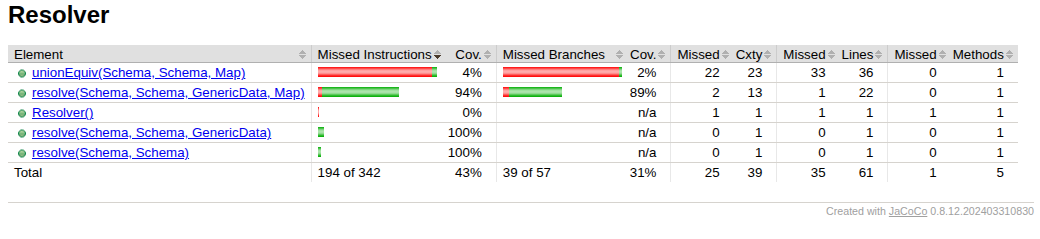
\includegraphics[width=0.85\textwidth]{immagini/jacocoresolver.png}
\caption{Report JaCoCo della suite manuale su \texttt{Resolver}.}
\label{fig:jacoco-resolver-bb}
\end{figure}

\begin{figure}[h]
\centering
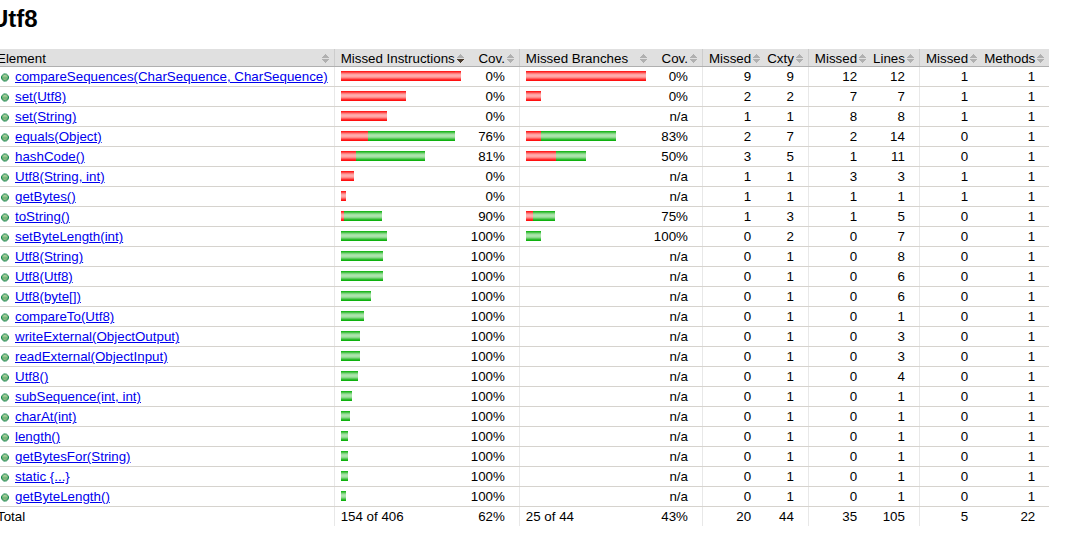
\includegraphics[width=0.85\textwidth]{immagini/jacocoutf8.png}
\caption{Report JaCoCo della suite manuale su \texttt{Utf8}.}
\label{fig:jacoco-utf8-bb}
\end{figure}
\begin{table}[h]
\centering
\footnotesize
\begin{tabular}{lcccc}
\toprule
\textbf{Classe} & \textbf{Test generati} & \textbf{Error-revealing} & \textbf{Statement Cov.} & \textbf{Branch Cov.} \\
\midrule
\texttt{Resolver} & 3508 & 0 & 1.6\% & 0\% \\
\texttt{Utf8} & 2841 & 0 & 79\% & 75\% \\
\bottomrule
\end{tabular}
\caption{Risultati della generazione con Randoop (budget 60s), coverage isolata per classe.}
\label{tab:randoop-results}
\end{table}
\begin{figure}[h]
\centering
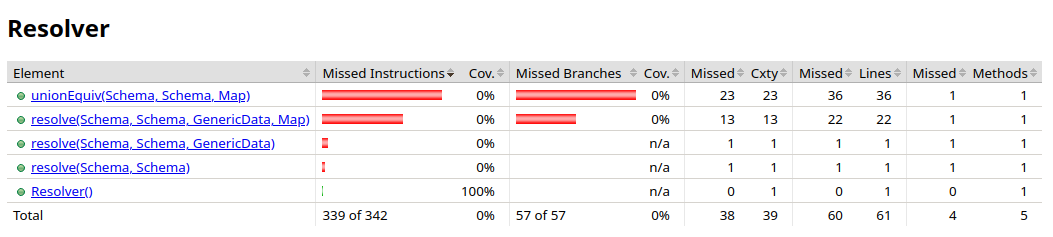
\includegraphics[width=0.85\textwidth]{immagini/randoopresolver.png}
\caption{Report JaCoCo della suite Randoop isolata su \texttt{Resolver}.}
\label{fig:jacoco-resolver-randoop}
\end{figure}
\begin{table}[h]
\centering
\begin{minipage}{0.95\textwidth}
\begin{quote}
\ttfamily\small
\textbf{Prompt 1 -- Zero-shot senza codice sorgente:}\\[4pt]
Scrivi test JUnit 5 per il metodo statico Resolver.resolve(Schema writer, Schema reader)
della libreria Apache Avro (package org.apache.avro). Non fornirò il codice sorgente:
basati solo sulla tua conoscenza di Avro e della sua logica di schema resolution.
\end{quote}

\begin{quote}
\ttfamily\small
\textbf{Prompt 2 -- Zero-shot con codice sorgente:}\\[4pt]
Scrivi test JUnit 5 per la seguente classe Java. Copri tutti i casi che ritieni rilevanti.\\[4pt]
{[}codice sorgente completo di Resolver.java{]}
\end{quote}

\begin{quote}
\ttfamily\small
\textbf{Prompt 3 -- Con vincoli di progetto espliciti:}\\[4pt]
Scrivi test JUnit 5 per la classe Resolver di Apache Avro (codice sotto).
Segui queste regole:\\
- package org.apache.avro\\
- niente wildcard import, solo import espliciti\\
- indentazione a 2 spazi (il progetto usa Spotless con questa configurazione)\\
- NON usare @Nested: la configurazione Surefire di questo progetto esclude le classi
  interne (pattern **{/}*\$*), quindi tutti i metodi @Test devono stare in
  un'unica classe a livello singolo\\
- copri sistematicamente queste categorie di risoluzione schema writer/reader:
  tipi primitivi uguali (DoNothing), promozioni numeriche valide (Promote),
  combinazioni incompatibili (ErrorAction), FIXED (nome/size uguali o diversi),
  ARRAY/MAP (Container), ENUM (simboli uguali o nome diverso),
  RECORD (campi aggiunti/rimossi, con o senza default),
  UNION (solo lato reader, solo lato writer)\\
- per ogni test aggiungi un commento breve su quale categoria copre\\[4pt]
{[}codice sorgente completo di Resolver.java{]}
\end{quote}
\end{minipage}
\caption{Testo completo dei tre prompt utilizzati per la generazione LLM su \texttt{Resolver}.}
\label{tab:prompt-resolver}
\end{table}
\begin{figure}[h]
\centering
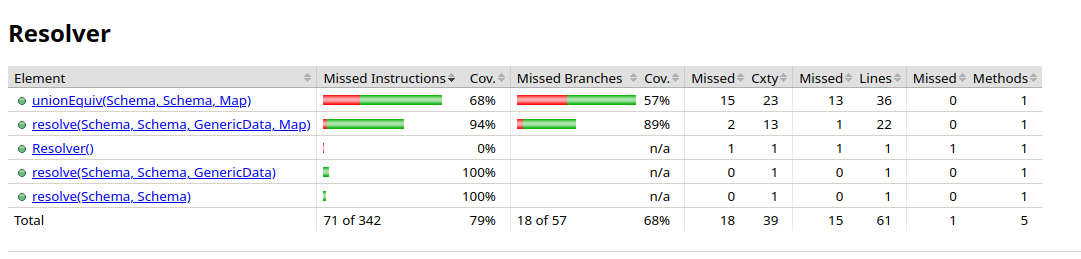
\includegraphics[width=0.85\textwidth]{immagini/llmresolver.png}
\caption{Report JaCoCo della suite LLM (Prompt 2+3) isolata su \texttt{Resolver}.}
\label{fig:jacoco-resolver-llm}
\end{figure}\begin{table}[h]
\centering
\footnotesize
\begin{tabular}{lccc}
\toprule
\textbf{Prompt} & \textbf{Test generati} & \textbf{Esito} & \textbf{Interventi manuali} \\
\midrule
1 (senza codice) & -- & Non compilabile & N/A \\
2 (con codice) & 45 & 45/45 passanti & Appiattimento \texttt{@Nested} \\
3 (con vincoli) & 13 & 13/13 passanti & Nessuno \\
\bottomrule
\end{tabular}
\caption{Risultati dei tre prompt LLM (Gemini) su \texttt{Resolver}.}
\label{tab:llm-resolver-results}
\end{table}

\begin{table}[h]
\centering
\footnotesize
\begin{tabular}{lc}
\toprule
\textbf{Metrica} & \textbf{Valore} \\
\midrule
Test generati & 78 \\
Statement coverage (JaCoCo) & 88.5\% \\
Branch coverage (JaCoCo) & 84.2\% \\
\bottomrule
\end{tabular}
\caption{Risultati della generazione EvoSuite su \texttt{Resolver} (budget 60s), copertura misurata con JaCoCo sulla suite isolata.}
\label{tab:evosuite-resolver}
\end{table}
\begin{figure}[h]
\centering
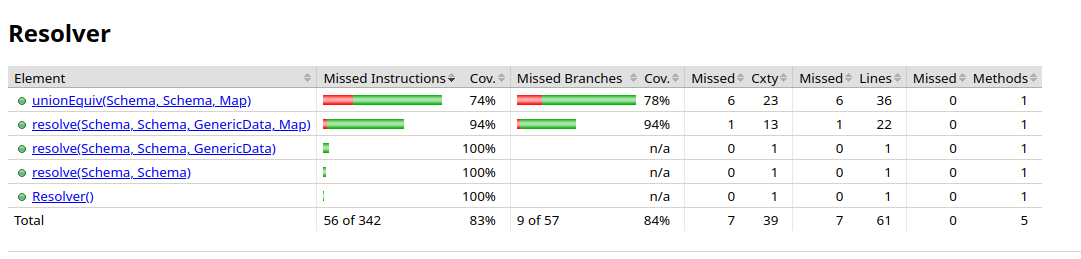
\includegraphics[width=0.85\textwidth]{immagini/evosuiteresolver.png}
\caption{Report JaCoCo della suite EvoSuite isolata su \texttt{Resolver}.}
\label{fig:jacoco-resolver-evosuite}
\end{figure}

\begin{figure}[h]
\centering
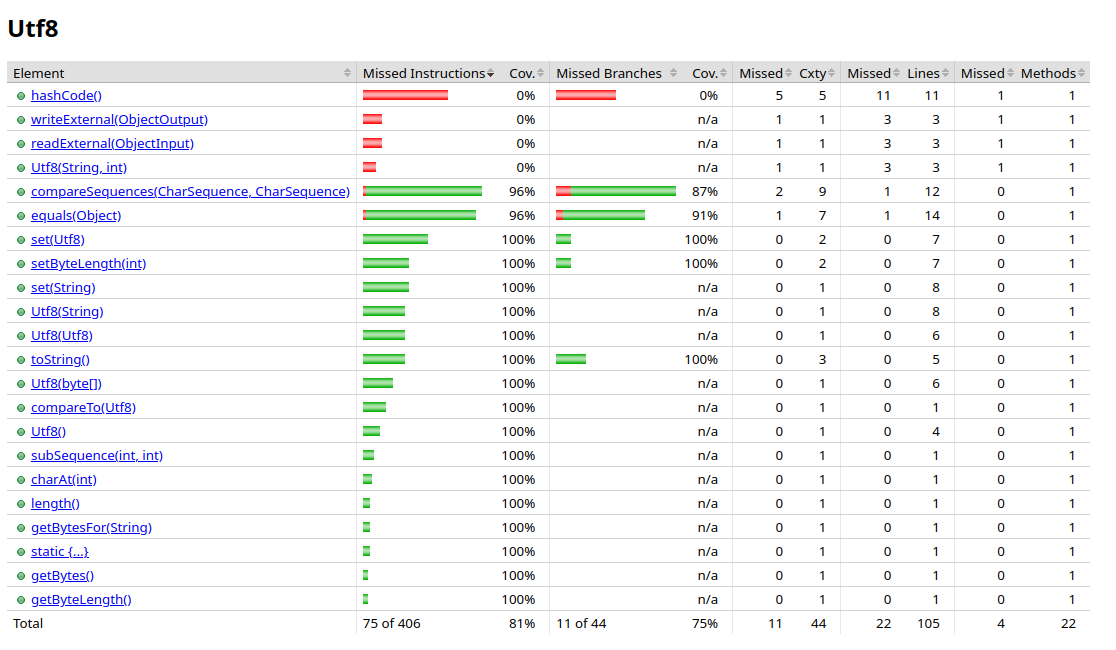
\includegraphics[width=0.85\textwidth]{immagini/randooputf8.png}
\caption{Report JaCoCo della suite Randoop isolata su \texttt{Utf8}.}
\label{fig:jacoco-utf8-randoop}
\end{figure}

\begin{figure}[h]
\centering
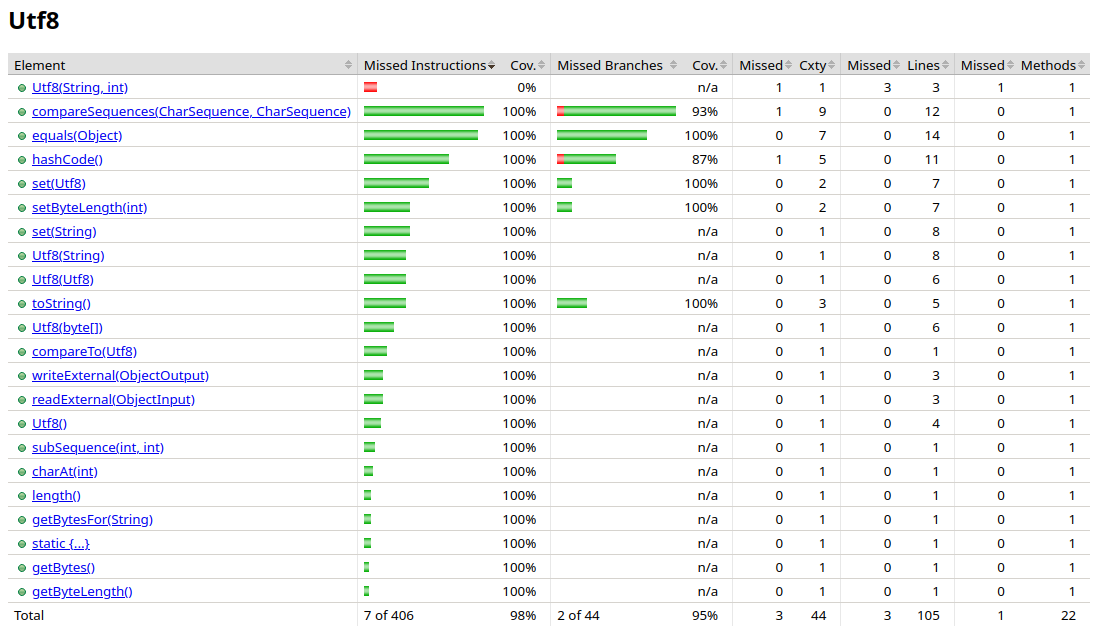
\includegraphics[width=0.85\textwidth]{immagini/llmutf8.png}
\caption{Report JaCoCo della suite LLM (Prompt 2+3) isolata su \texttt{Utf8}.}
\label{fig:jacoco-utf8-llm}
\end{figure}

\begin{table}[h]
\centering
\begin{minipage}{0.95\textwidth}
\begin{quote}
\ttfamily\small
\textbf{Prompt 1 -- Zero-shot senza codice sorgente:}\\[4pt]
Scrivi test JUnit 5 per la classe Utf8 della libreria Apache Avro (package org.apache.avro.util).
La classe rappresenta una sequenza di byte codificata UTF-8, con metodi per impostare/ottenere
lunghezza e contenuto in byte, confronto e conversione a String. Non fornirò il codice sorgente:
basati solo sulla tua conoscenza di Avro e del formato UTF-8.
\end{quote}

\begin{quote}
\ttfamily\small
\textbf{Prompt 2 -- Zero-shot con codice sorgente:}\\[4pt]
Scrivi test JUnit 5 per la seguente classe Java. Copri tutti i casi che ritieni rilevanti.\\[4pt]
{[}codice sorgente completo di Utf8.java{]}
\end{quote}

\begin{quote}
\ttfamily\small
\textbf{Prompt 3 -- Con vincoli di progetto espliciti:}\\[4pt]
Scrivi test JUnit 5 per la classe Utf8 di Apache Avro (codice sotto).
Segui queste regole:\\
- package org.apache.avro.util\\
- niente wildcard import, solo import espliciti\\
- indentazione a 2 spazi (il progetto usa Spotless con questa configurazione)\\
- NON usare @Nested: la configurazione Surefire di questo progetto esclude le classi
  interne (pattern **{/}*\$*), quindi tutti i metodi @Test devono stare in
  un'unica classe a livello singolo\\
- copri sistematicamente: costruttori (vuoto, da String, da byte[], da altro Utf8),
  getBytes/setBytes, getByteLength/setByteLength (inclusa l'espansione E la riduzione
  dell'array interno), equals/hashCode, compareTo, toString, casi limite come stringhe
  vuote o con caratteri multi-byte UTF-8\\
- per ogni test aggiungi un commento breve su cosa copre\\[4pt]
{[}codice sorgente completo di Utf8.java{]}
\end{quote}
\end{minipage}
\caption{Testo completo dei tre prompt utilizzati per la generazione LLM su \texttt{Utf8}.}
\label{tab:prompt-utf8}
\end{table}

\begin{table}[h]
\centering
\footnotesize
\begin{tabular}{lccc}
\toprule
\textbf{Prompt} & \textbf{Test generati} & \textbf{Esito} & \textbf{Interventi manuali} \\
\midrule
1 (senza codice) & -- & Nessuna allucinazione evidente & N/A (non integrato) \\
2 (con codice) & 23 & 23/23 passanti & Appiattimento \texttt{@Nested} \\
3 (con vincoli) & 17 & 16/16 passanti & Rimozione di 1 test (costruttore package-private) \\
\bottomrule
\end{tabular}
\caption{Risultati dei tre prompt LLM (Gemini) su \texttt{Utf8}.}
\label{tab:llm-utf8-results}
\end{table}

\begin{table}[h]
\centering
\footnotesize
\begin{tabular}{lc}
\toprule
\textbf{Metrica} & \textbf{Valore} \\
\midrule
Test generati & 63 \\
Statement coverage (JaCoCo) & 95.2\% \\
Branch coverage (JaCoCo) & 95.5\% \\
\bottomrule
\end{tabular}
\caption{Risultati della generazione EvoSuite su \texttt{Utf8} (budget 60s), copertura misurata con JaCoCo sulla suite isolata.}
\label{tab:evosuite-utf8}
\end{table}

\begin{figure}[h]
\centering
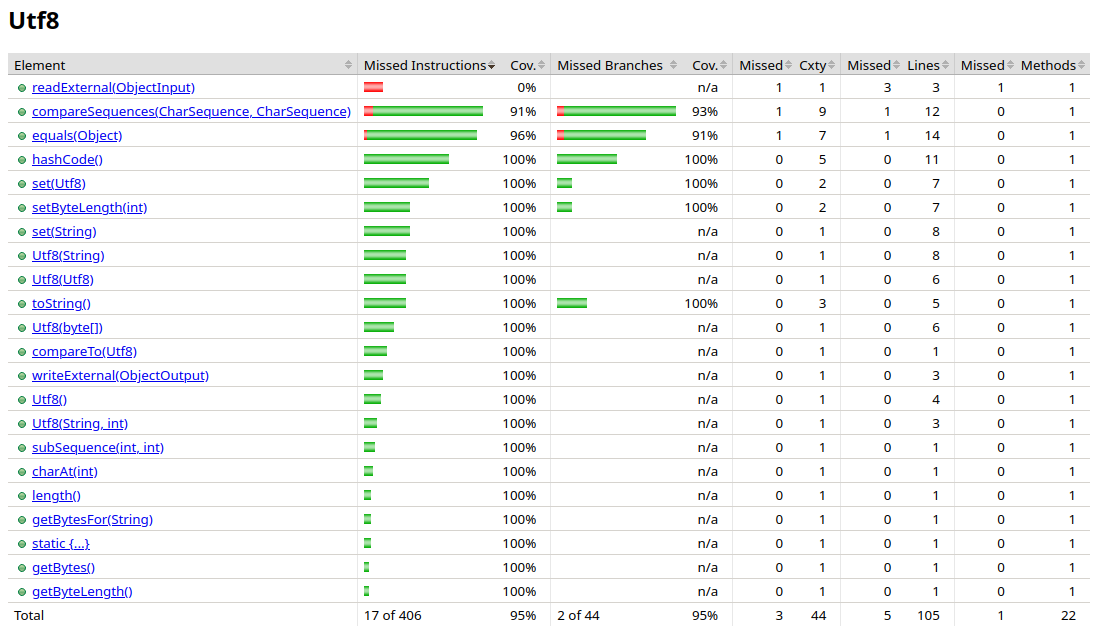
\includegraphics[width=0.85\textwidth]{immagini/evosuiteutf8.png}
\caption{Report JaCoCo della suite EvoSuite isolata su \texttt{Utf8}.}
\label{fig:jacoco-utf8-evosuite}
\end{figure}

\begin{table}[h]
\centering
\footnotesize
\begin{tabular}{llcc}
\toprule
\textbf{Famiglia} & \textbf{Classe} & \textbf{Statement Coverage} & \textbf{Branch Coverage} \\
\midrule
BB & \texttt{Resolver} & 42.6\% (26/61) & 31.6\% (18/57) \\
BB & \texttt{Utf8} & 66.7\% (70/105) & 43.2\% (19/44) \\
RND & \texttt{Resolver} & 1.6\% (1/61) & 0.0\% (0/57) \\
RND & \texttt{Utf8} & 79.0\% (83/105) & 75.0\% (33/44) \\
LLM & \texttt{Resolver} & 75.4\% (46/61) & 68.4\% (39/57) \\
LLM & \texttt{Utf8} & 97.1\% (102/105) & 95.5\% (42/44) \\
ES & \texttt{Resolver} & 88.5\% (54/61) & 84.2\% (48/57) \\
ES & \texttt{Utf8} & 95.2\% (100/105) & 95.5\% (42/44) \\
\bottomrule
\end{tabular}
\caption{Confronto di adeguatezza (Statement/Branch coverage) tra le quattro famiglie di test, per ciascuna classe.}
\label{tab:adeguatezza-confronto}
\end{table}
\begin{figure}[h]
\centering
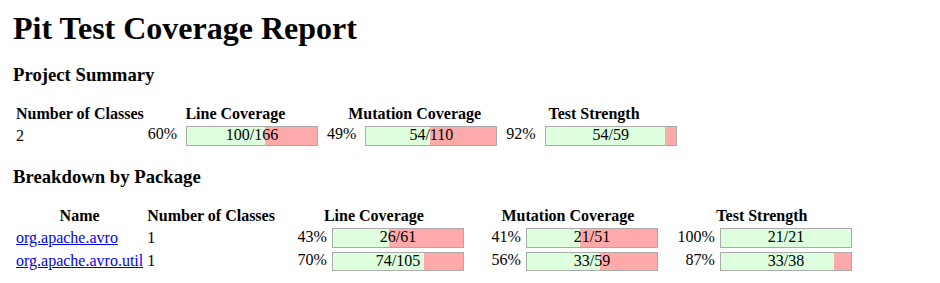
\includegraphics[width=0.85\textwidth]{immagini/pitreport.png}
\caption{Report PIT (indice generale), dopo l'integrazione dei test MT su \texttt{Utf8}.}
\label{fig:pit-report}
\end{figure}

\begin{table}[h]
\centering
\footnotesize
\begin{tabular}{lccc}
\toprule
\textbf{Classe} & \textbf{Line Coverage} & \textbf{Mutation Coverage} & \textbf{Test Strength} \\
\midrule
\texttt{Resolver} (suite BB) & 43\% (26/61) & 41\% (21/51) & 100\% (21/21) \\
\texttt{Utf8} (suite BB) & 67\% (70/105) & 37\% (22/59) & 65\% (22/34) \\
\texttt{Utf8} (suite BB + MT) & 70\% (74/105) & 56\% (33/59) & 87\% (33/38) \\
\bottomrule
\end{tabular}
\caption{Risultati del mutation testing con PIT, prima e dopo l'integrazione dei test MT su \texttt{Utf8}.}
\label{tab:pit-results}
\end{table}

\begin{table}[h]
\centering
\footnotesize
\begin{tabular}{lcccc}
\toprule
\textbf{Variante} & \textbf{BB} & \textbf{RND (campione)} & \textbf{LLM} & \textbf{ES} \\
\midrule
C1 & FAIL (compilazione) & FAIL (stesso motivo) & FAIL (stesso motivo) & PASS 78/78 \\
C2 & PASS 32/32 & PASS 500/500 & PASS 45+13/45+13 & PASS 78/78 \\
C3 & PASS 32/32 & PASS 500/500 & PASS 45+13/45+13 & PASS 78/78 \\
C4 & PASS 32/32 & PASS 500/500 & PASS 45+13/45+13 & PASS 78/78 \\
\bottomrule
\end{tabular}
\caption{Validazione delle famiglie di test su ciascuna variante di \texttt{Resolver}.}
\label{tab:resolver-refactor-passfail}
\end{table}

\begin{table}[h]
\centering
\footnotesize
\begin{tabular}{lccccc}
\toprule
\textbf{Metrica} & \textbf{C0} & \textbf{C1} & \textbf{C2} & \textbf{C3} & \textbf{C4} \\
\midrule
Statement Coverage & 92.3\% & 84.7\%$^1$ & 93.1\% & 92.2\% & 92.2\% \\
Branch Coverage & 83.6\% & 68.1\%$^1$ & 83.8\% & 82.8\% & 82.8\% \\
Mutation Score & 51\% & N/A$^2$ & 51\% & 51\% & 51\% \\
LOC (proxy smell) & 505 & 457 & 457 & 485 & 485 \\
Punti di decisione & 191 & 163 & 163 & 179 & 179 \\
\bottomrule
\end{tabular}
\caption{Delta di coverage, mutation score e proxy di smell tra C0 e le varianti C1-C4 di \texttt{Resolver}. $^1$C1 misurato solo su ES (unica famiglia compilante), non comparabile 1:1. $^2$Non misurabile: BB/RND/LLM non compilano contro C1, ES incompatibile con PIT.}
\label{tab:resolver-refactor-delta}
\end{table}
\begin{table}[h]
\centering
\footnotesize
\begin{tabular}{lccccc}
\toprule
\textbf{Famiglia} & \textbf{C1} & \textbf{C2} & \textbf{C3} & \textbf{C4} \\
\midrule
BB (35 test) & PASS 35/35 & PASS 35/35 & PASS 35/35 & PASS 35/35 \\
MT (14 test) & FAIL 13/14 & FAIL 13/14 & PASS 14/14 & PASS 14/14 \\
RND (campione 500) & FAIL (compilazione) & PASS 500/500 & PASS 500/500 & PASS 500/500 \\
LLM (Prompt 2+3) & FAIL (compilazione) & PASS 23+17/23+17 & PASS 23+17/23+17 & PASS 23+17/23+17 \\
ES (63 test) & FAIL (compilazione) & FAIL 61/63 & PASS 63/63 & FAIL 62/63 \\
\bottomrule
\end{tabular}
\caption{Validazione delle cinque famiglie di test su ciascuna variante di \texttt{Utf8}.}
\label{tab:utf8-refactor-passfail}
\end{table}

\begin{table}[h]
\centering
\footnotesize
\begin{tabular}{lccccc}
\toprule
\textbf{Metrica} & \textbf{C0} & \textbf{C1} & \textbf{C2} & \textbf{C3} & \textbf{C4} \\
\midrule
Statement Coverage & 100\% & 68.7\%$^1$ & 100\% & 100\% & 100\% \\
Branch Coverage & 97.7\% & 47.2\%$^1$ & 97.2\% & 97.7\% & 97.5\% \\
Mutation Score & 86\% & N/A$^2$ & N/A$^2$ & 86\% & 85\% \\
LOC (proxy smell) & 178 & 172 & 172 & 177 & 175 \\
Punti di decisione & 27 & 24 & 24 & 27 & 25 \\
\bottomrule
\end{tabular}
\caption{Delta di coverage, mutation score e proxy di smell tra C0 e le varianti C1-C4 di \texttt{Utf8}. $^1$Misurato solo su BB+MT (2 famiglie su 5). $^2$PIT rifiuta l'esecuzione: la suite MT non è verde su C1/C2.}
\label{tab:utf8-refactor-delta}
\end{table}

\begin{table}[h]
\centering
\footnotesize
\begin{tabular}{p{2.2cm}p{4.4cm}p{6.4cm}}
\toprule
\textbf{Famiglia} & \textbf{Naming dei metodi di test} & \textbf{Evidenza osservata nel codice generato} \\
\midrule
BB / MT & Descrittivo, per categoria (es. \texttt{testSetByteLengthAumento}) & Scritti manualmente; commento di intento su ogni test \\
LLM (Prompt 2--3) & Descrittivo (es. \texttt{testSetByteLengthExpansion}, \texttt{testCopyConstructor}) & \texttt{@DisplayName} in linguaggio naturale; commento di categoria per test (Prompt 3) \\
Randoop & Sequenziale (\texttt{test0001}, \texttt{test0002}, \dots) & Commenti solo automatici (``\emph{The following exception was thrown during execution...}''), non di intento \\
EvoSuite & Sequenziale (\texttt{test00}, \texttt{test01}, \dots) & Nessun commento descrittivo; input spesso stringhe casuali prive di significato (es. \texttt{"-5.6D8[[?\%/nW,u\#G"}) \\
\bottomrule
\end{tabular}
\caption{Caratterizzazione qualitativa della leggibilità dei test prodotti da ciascuna famiglia, basata su ispezione diretta del codice sorgente generato in entrambe le classi.}
\label{tab:test-clarity}
\end{table}

\end{document}